\documentclass[10pt]{beamer}

\usepackage[utf8]{inputenc}
\usepackage[english]{babel}
\usepackage[T1]{fontenc}

\usepackage{tabularx}  % pour les tableaux (taille des colonnes)
\usepackage{multirow}  % pour les tableaux (fusion des lignes)
\usepackage{amsmath,amsfonts,amssymb,amstext,amsthm}  % pour les équations

\usepackage{listings}  % pour afficher du code
% Mise en forme des légendes des listings
\renewcommand\lstlistingname{\darwin\color{bleuCNR} Algorithm}
\usepackage{appendixnumberbeamer}

\usepackage{booktabs}

\newcommand{\themename}{\textbf{\textsc{cnr }}}

% Use cnr theme with all possible options
\usetheme[
  imagecoverpath=barrage-roche-de-glun.jpg,
  imagecoveropacity=0.8,
  logo=cnr-engineering,
  hidesouslogo
]{cnr}

% Customize cover page
\defbeamertemplate*{title page}{}[1][]
{
  \vskip1.4cm

  \setbeamercolor{title page header}{fg=white,bg=black}
  \pgfsetfillopacity{0.3}
  \begin{beamercolorbox}[wd=11.5cm,sep=5pt,#1]{title page header}
    \pgfsetfillopacity{1}\centering\LARGE\darwin
    \usebeamerfont{title}\inserttitle\par
  \end{beamercolorbox}

  \vskip1.8cm

  \begin{beamercolorbox}[wd=11.5cm,leftskip=1cm,#1]{author}
    \begin{flushleft}
      \darwin
      \usebeamerfont{author}\insertdate \\[2pt]
      \usebeamerfont{author}\insertauthor
    \end{flushleft}
  \end{beamercolorbox}

  \vskip-0.2cm

  \begin{beamercolorbox}[wd=11.5cm,leftskip=1cm,#1]{subtitle}
    \begin{flushleft}
      {\darwin\color{white}\textit{\insertsubtitle}}
    \end{flushleft}
  \end{beamercolorbox}

  \vfill

  \setcounter{framenumber}{0}
}

\setbeamertemplate{caption}{\insertcaption}  % suppression numérotation des figures/tableaux


\title{TatooineMesher: Anisotropic interpolation from 1D cross-sections and 2D channel mesher}
\subtitle{Telemac User Conference 2019}
\date{17/09/2019, Toulouse (France)}
\author{\underline{L. DURON}, F.-X. CIERCO, K. SAAD}


\begin{document}


\maketitle


\begin{frame}{Table of contents}
  \tableofcontents
\end{frame}


%%%%%%%%%%%%%%%%%%%%%%%%%%%%%%%%%%%%%%%%%%%%%%%%%%%%%%%%%%%%%%%%%
\section{Introduction}

\begin{frame}{Introduction}

\paragraphtitle{CNR}
\begin{itemize}
    \item 1\textsuperscript{st} producer of exclusively renewable energy in France
    \begin{itemize}
        \item 18 hydroelectric facilities on the Rhône River (3000 MW)
        \item Solar and wind energy (1000 MW)
    \end{itemize}
    \item CNR Engineering Departement (for CNR and third party)
\end{itemize}

\pause

\paragraphtitle{Objectives}
\begin{enumerate}
    \item \textbf{pre-treatment 1D models}: interpolate intermediate
cross-sections
    \item \textbf{pre-treatment 2D models}: interpolate the bathymetry
and/or mesh the river bed
    \item \textbf{post-treatment 1D models}: visualize the results in 2D (in a projected geographic coordinate system)
\end{enumerate}

\end{frame}


\begin{frame}{Developed tools}

\begin{itemize}
    \item Code : Python 3
    \item Command line scripts
    \item Usage: \url{https://github.com/CNR-Engineering/TatooineMesher/wiki}
\end{itemize}

\vspace{0.2cm}
\pause

\paragraphtitle{Installation and requirements}

{\centering
\lstinputlisting[basicstyle=\tiny,
    language=bash, xleftmargin=0.05\textwidth, escapechar=@]{installation.sh}
}

PyTelTools and Crue10\_tools (contains Mascaret part of postel) are 2 packages required.

\end{frame}


%%%%%%%%%%%%%%%%%%%%%%%%%%%%%%%%%%%%%%%%%%%%%%%%%%%%%%%%%%%%%%%%%
\section{Mesh generation}

\subsection{Principle - Step by step}
\begin{frame}\frametitle{Principle - Step by step}

  \begin{columns}[T,]
    \column{0.43\textwidth}
      \begin{enumerate}
        \item<1-> Order cross-sections (CS)
        \item<2-> Intersect CS and constraint lines
        \item<3-> Generate nodes for each submesh
        \begin{enumerate}
            \item<4-> Linear interp. for intermediate CS
            \item<5-> Application of an affine transformation
            \item<6-> Lateral sampling
        \end{enumerate}
        \item<7-> Triangulate over the whole domain
        \item<8-> Definition of a flow-oriented coordinate system
      \end{enumerate}

    \column{0.42\textwidth}
    \begin{figure}[H]
        \vspace{-0.5cm}
        \only<1-3>{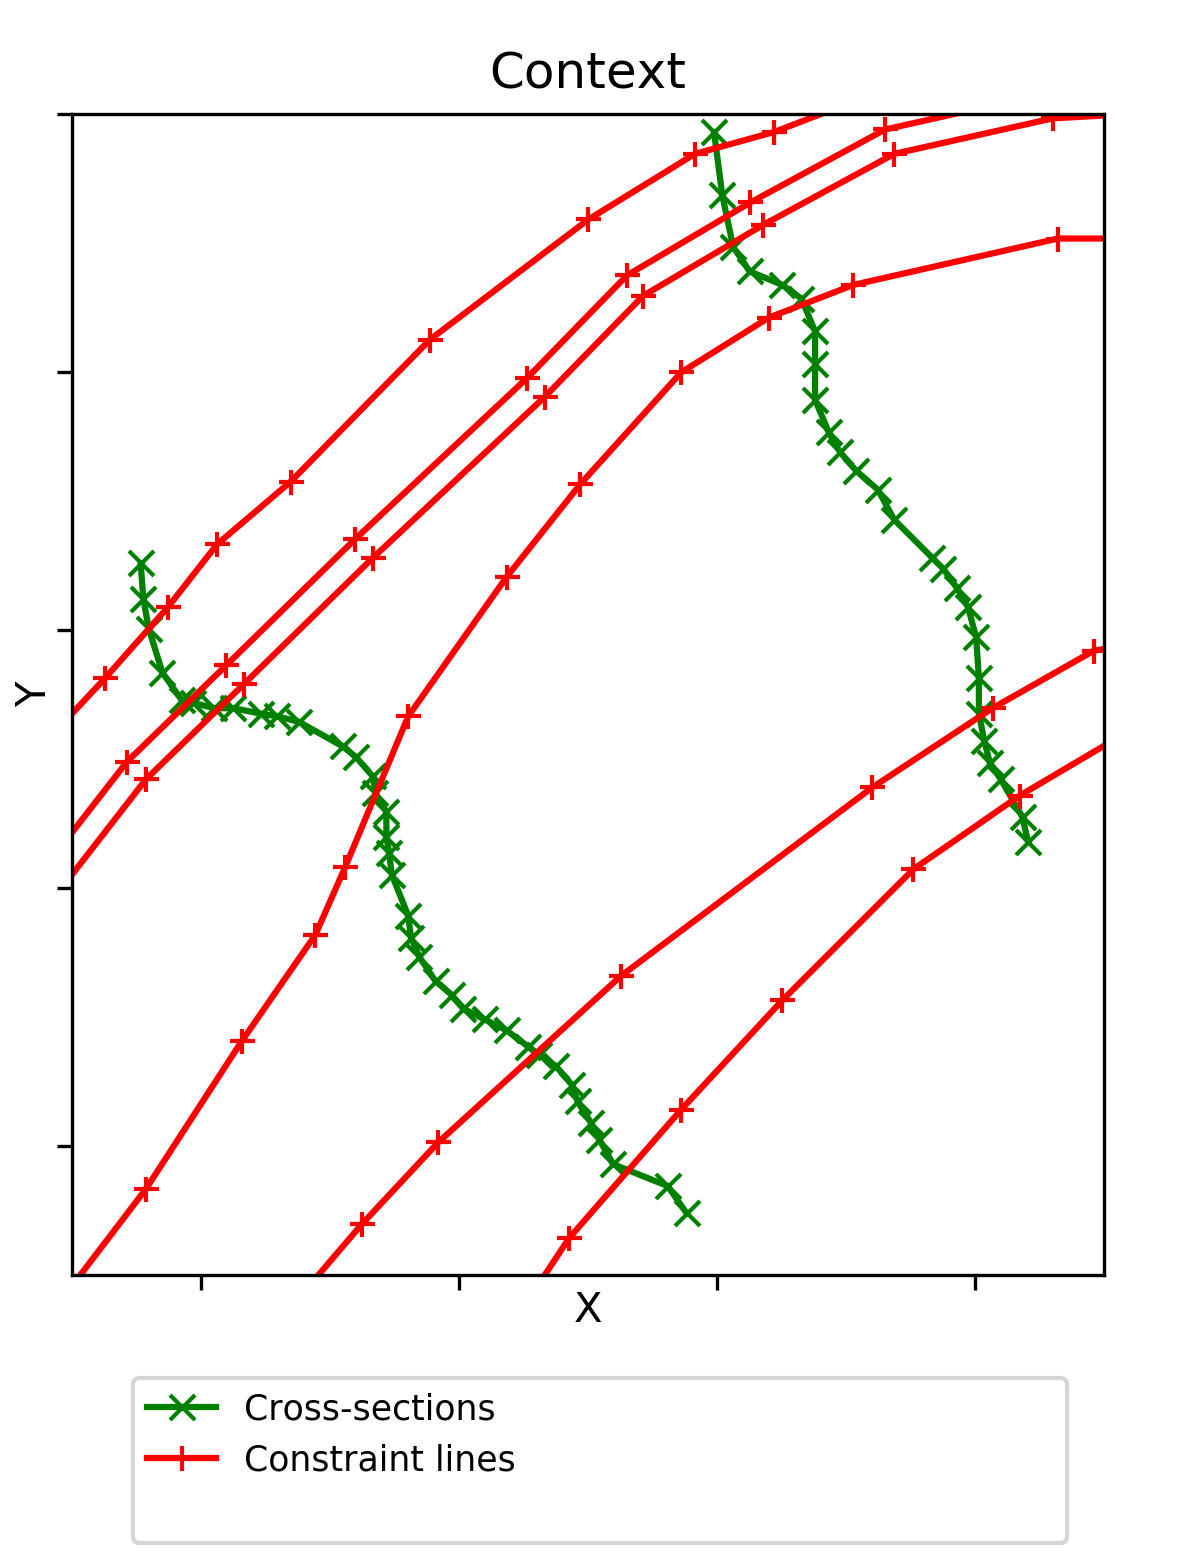
\includegraphics[width=5.5cm]{figures/plot_mesh_principle_0.png}}
        \only<4>{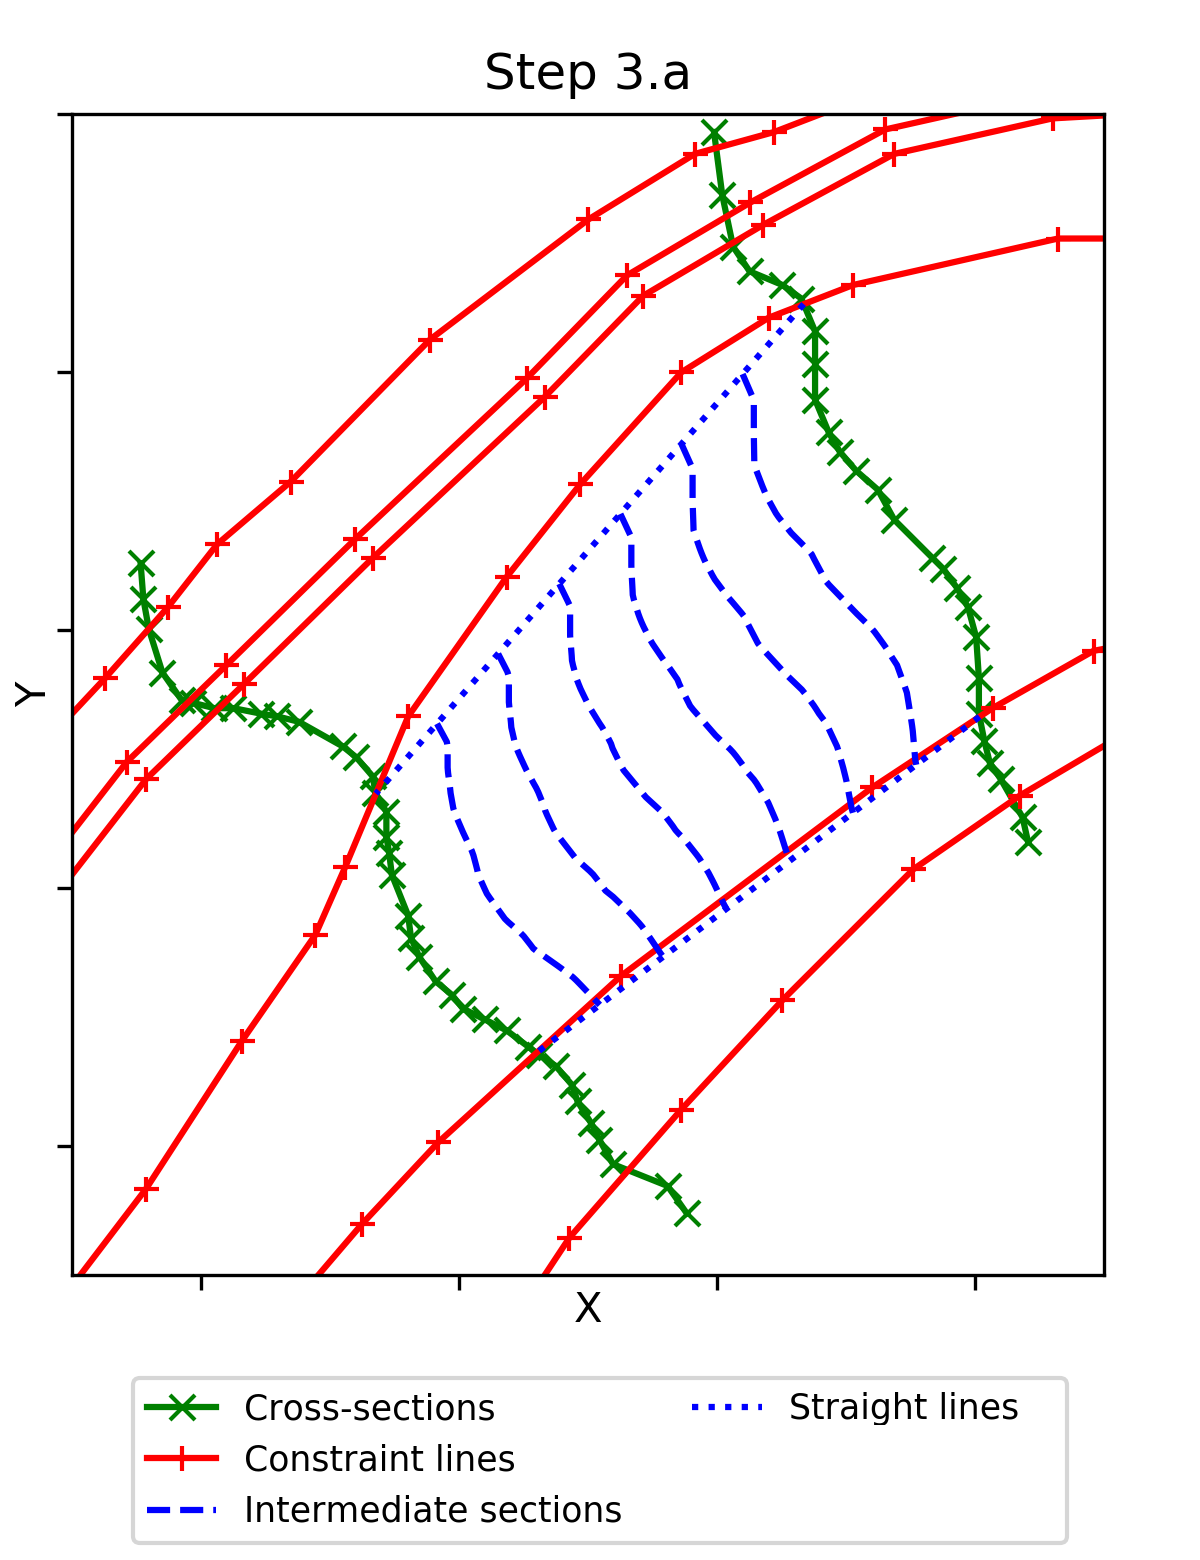
\includegraphics[width=5.5cm]{figures/plot_mesh_principle_1.png}}
        \only<5>{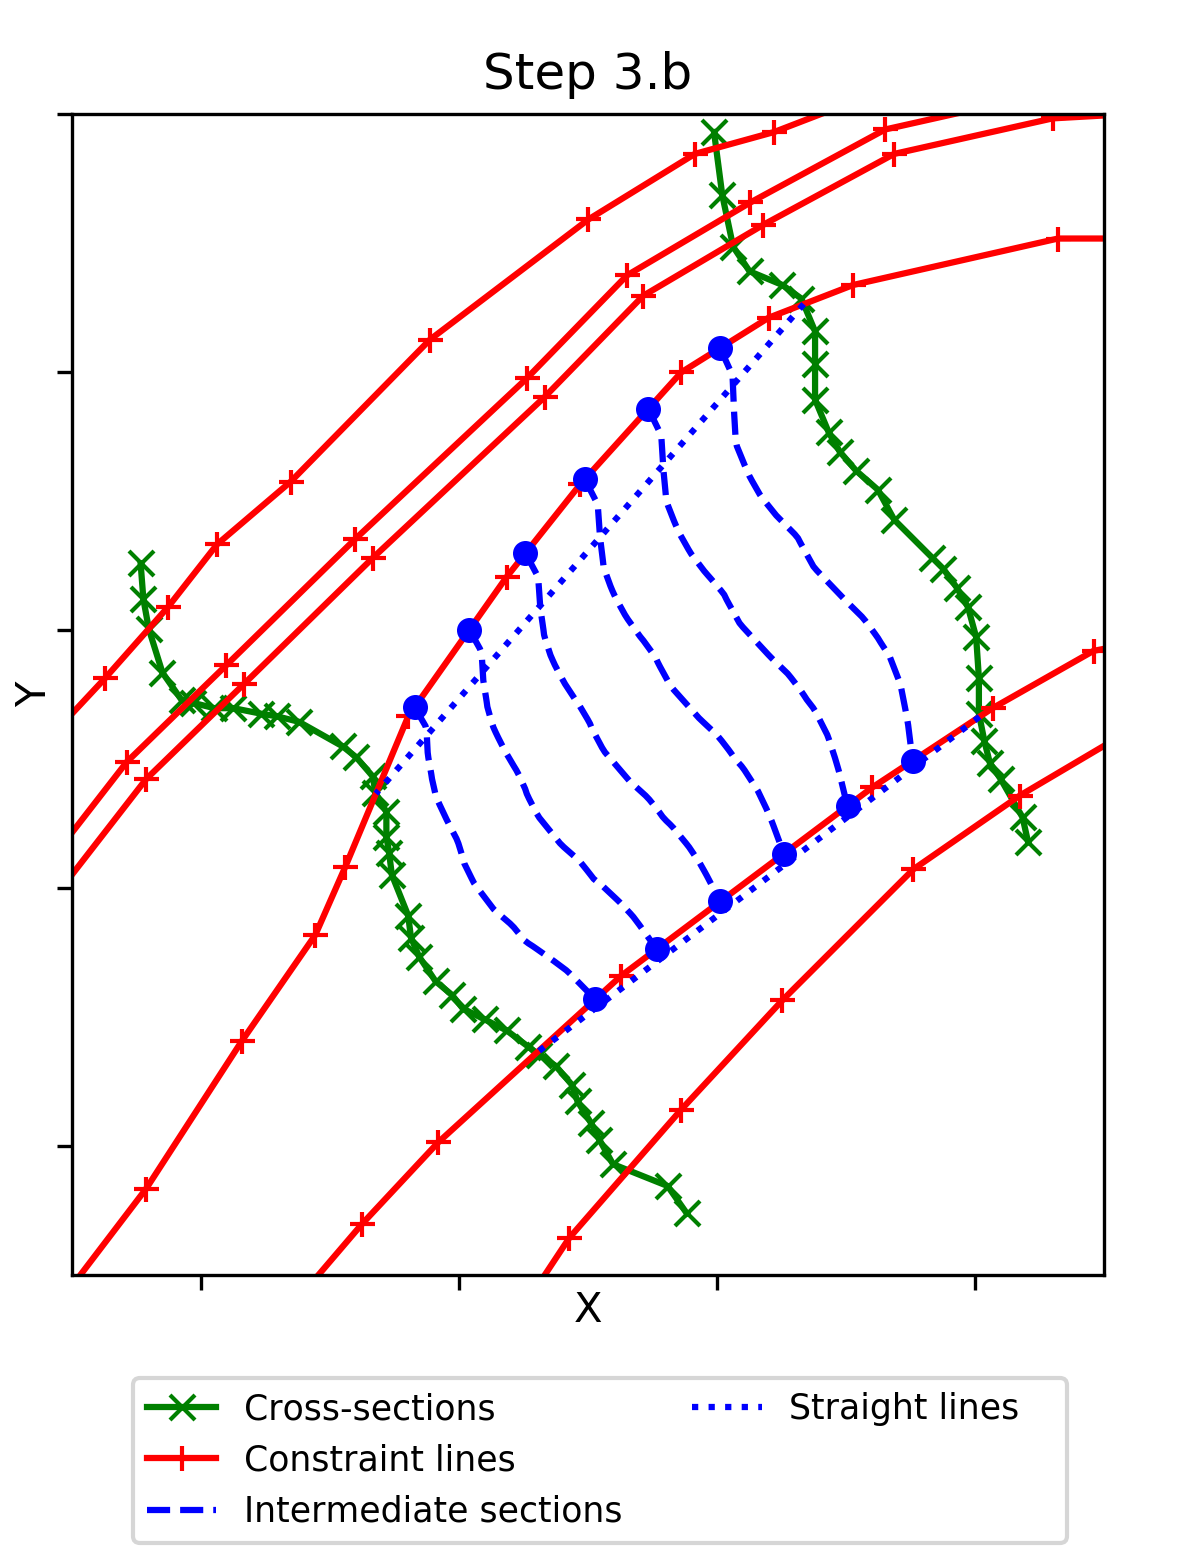
\includegraphics[width=5.5cm]{figures/plot_mesh_principle_2.png}}
        \only<6>{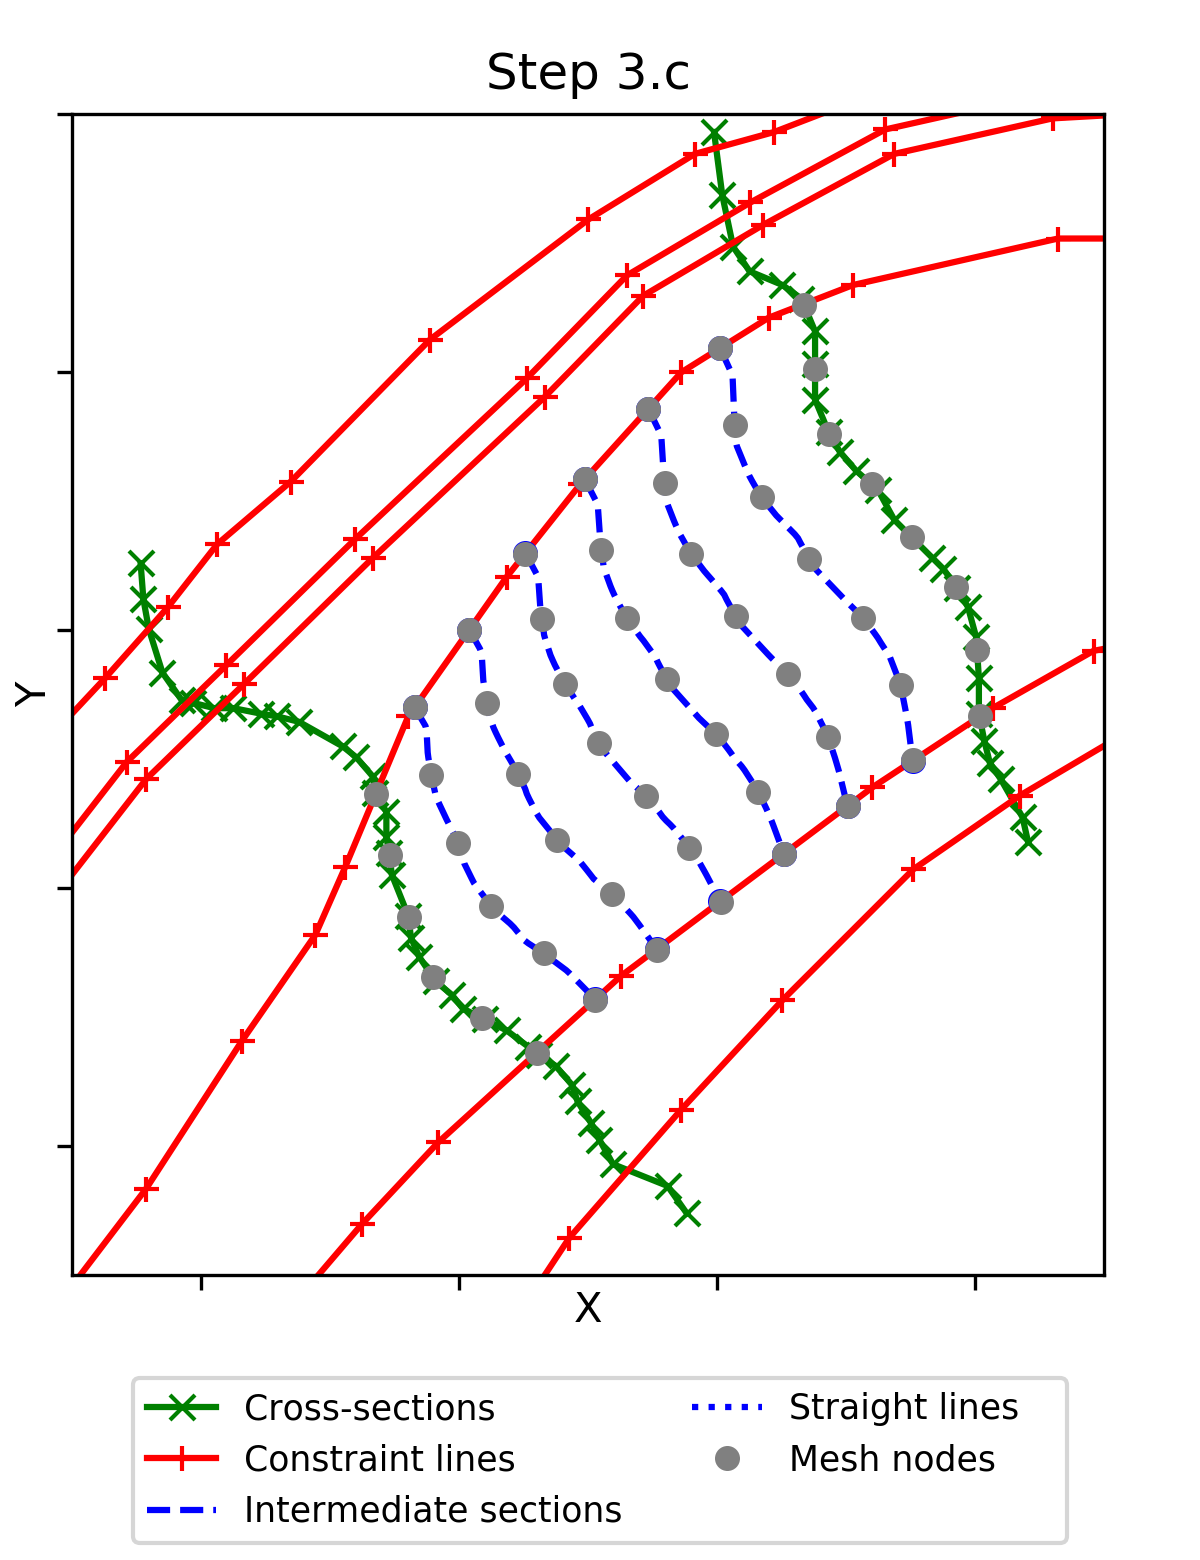
\includegraphics[width=5.5cm]{figures/plot_mesh_principle_3.png}}
        \only<7>{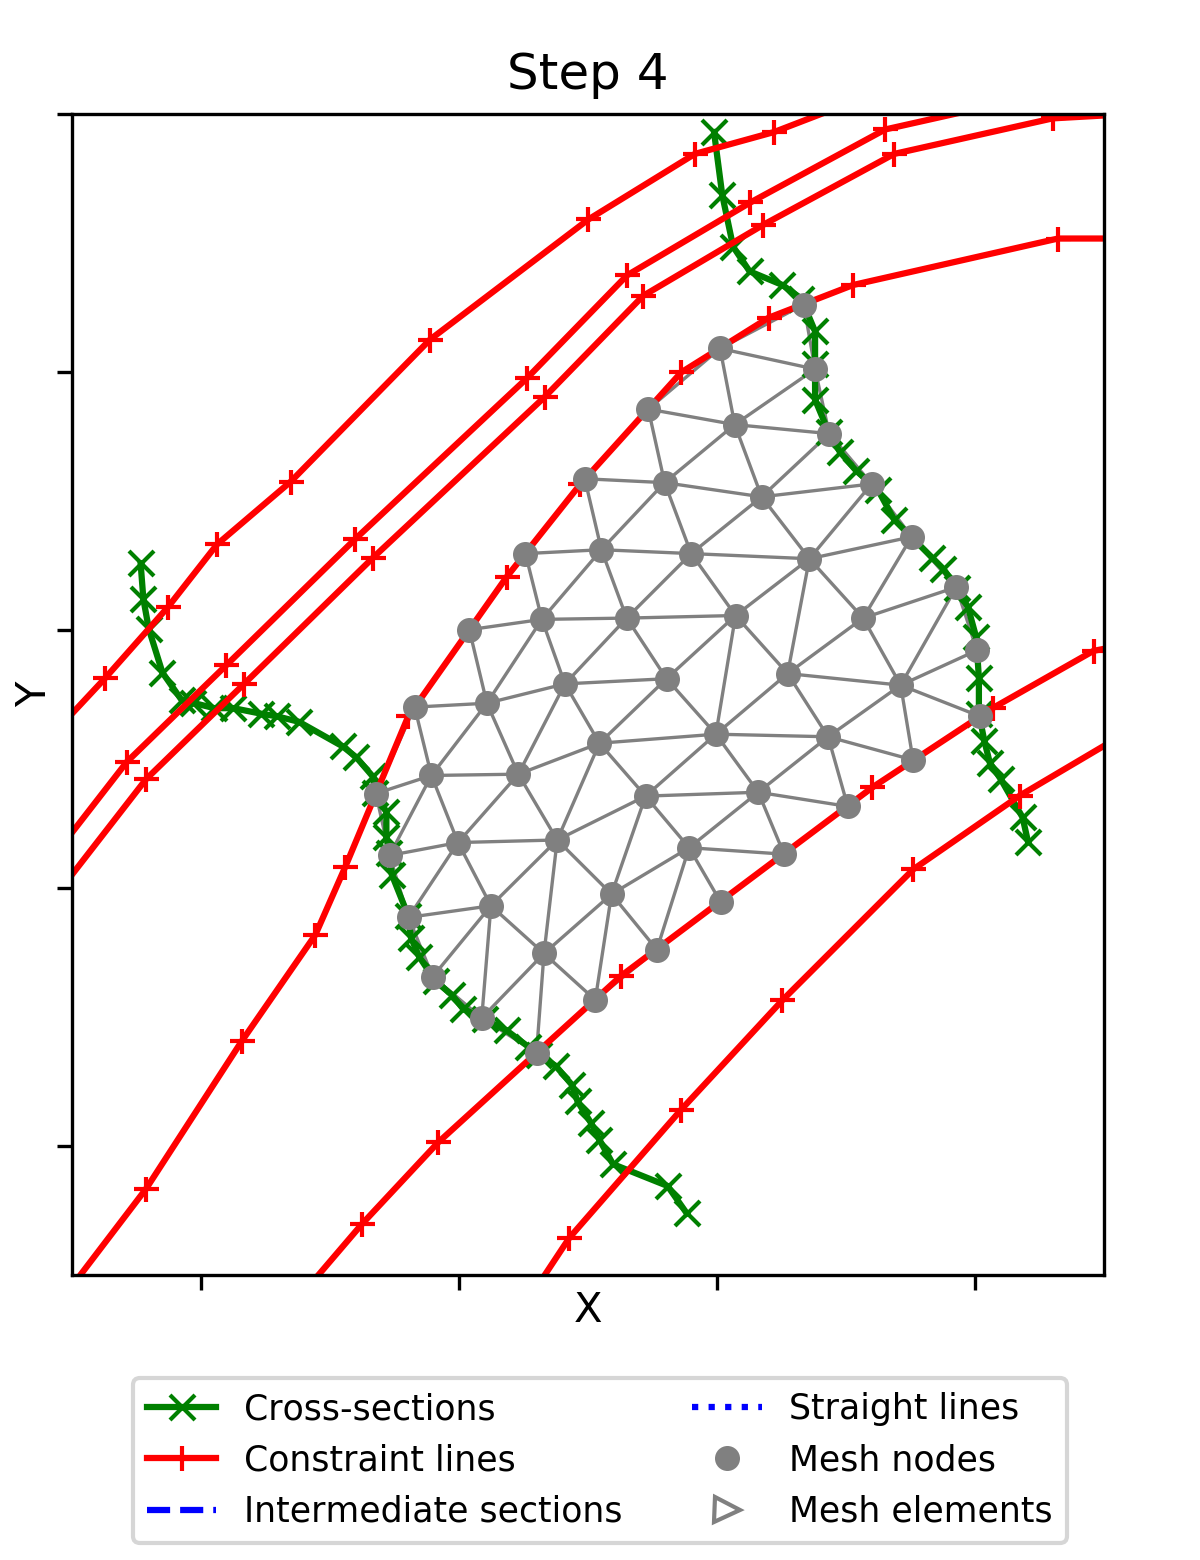
\includegraphics[width=5.5cm]{figures/plot_mesh_principle_4.png}}
        \only<8>{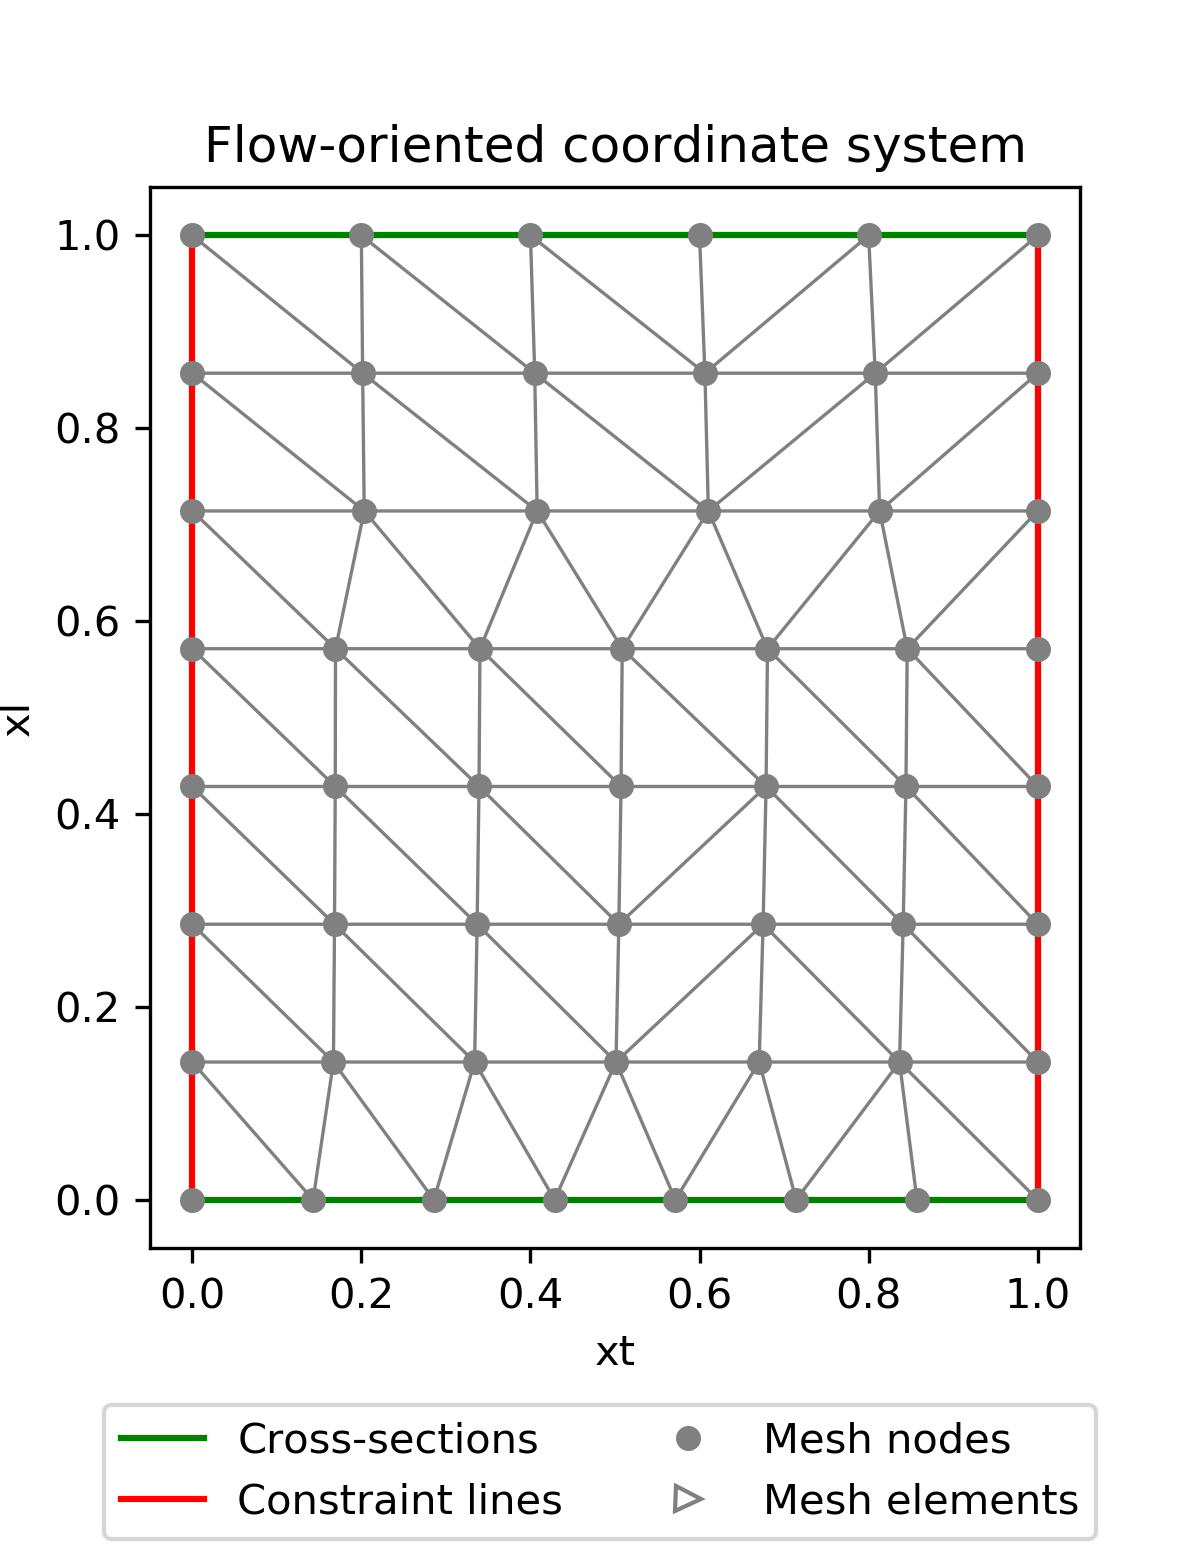
\includegraphics[width=5.5cm]{figures/plot_mesh_principle_5.png}}
    \end{figure}
  \end{columns}

\end{frame}


\subsection{Overview of main features}

\begin{frame}\frametitle{Feature 1 : Spatial discretization}

\begin{itemize}
    \item Longitudinal discretization
    \item Lateral discretization : structured or not (figure below)
\end{itemize}

\begin{figure}[H]
    \centerline{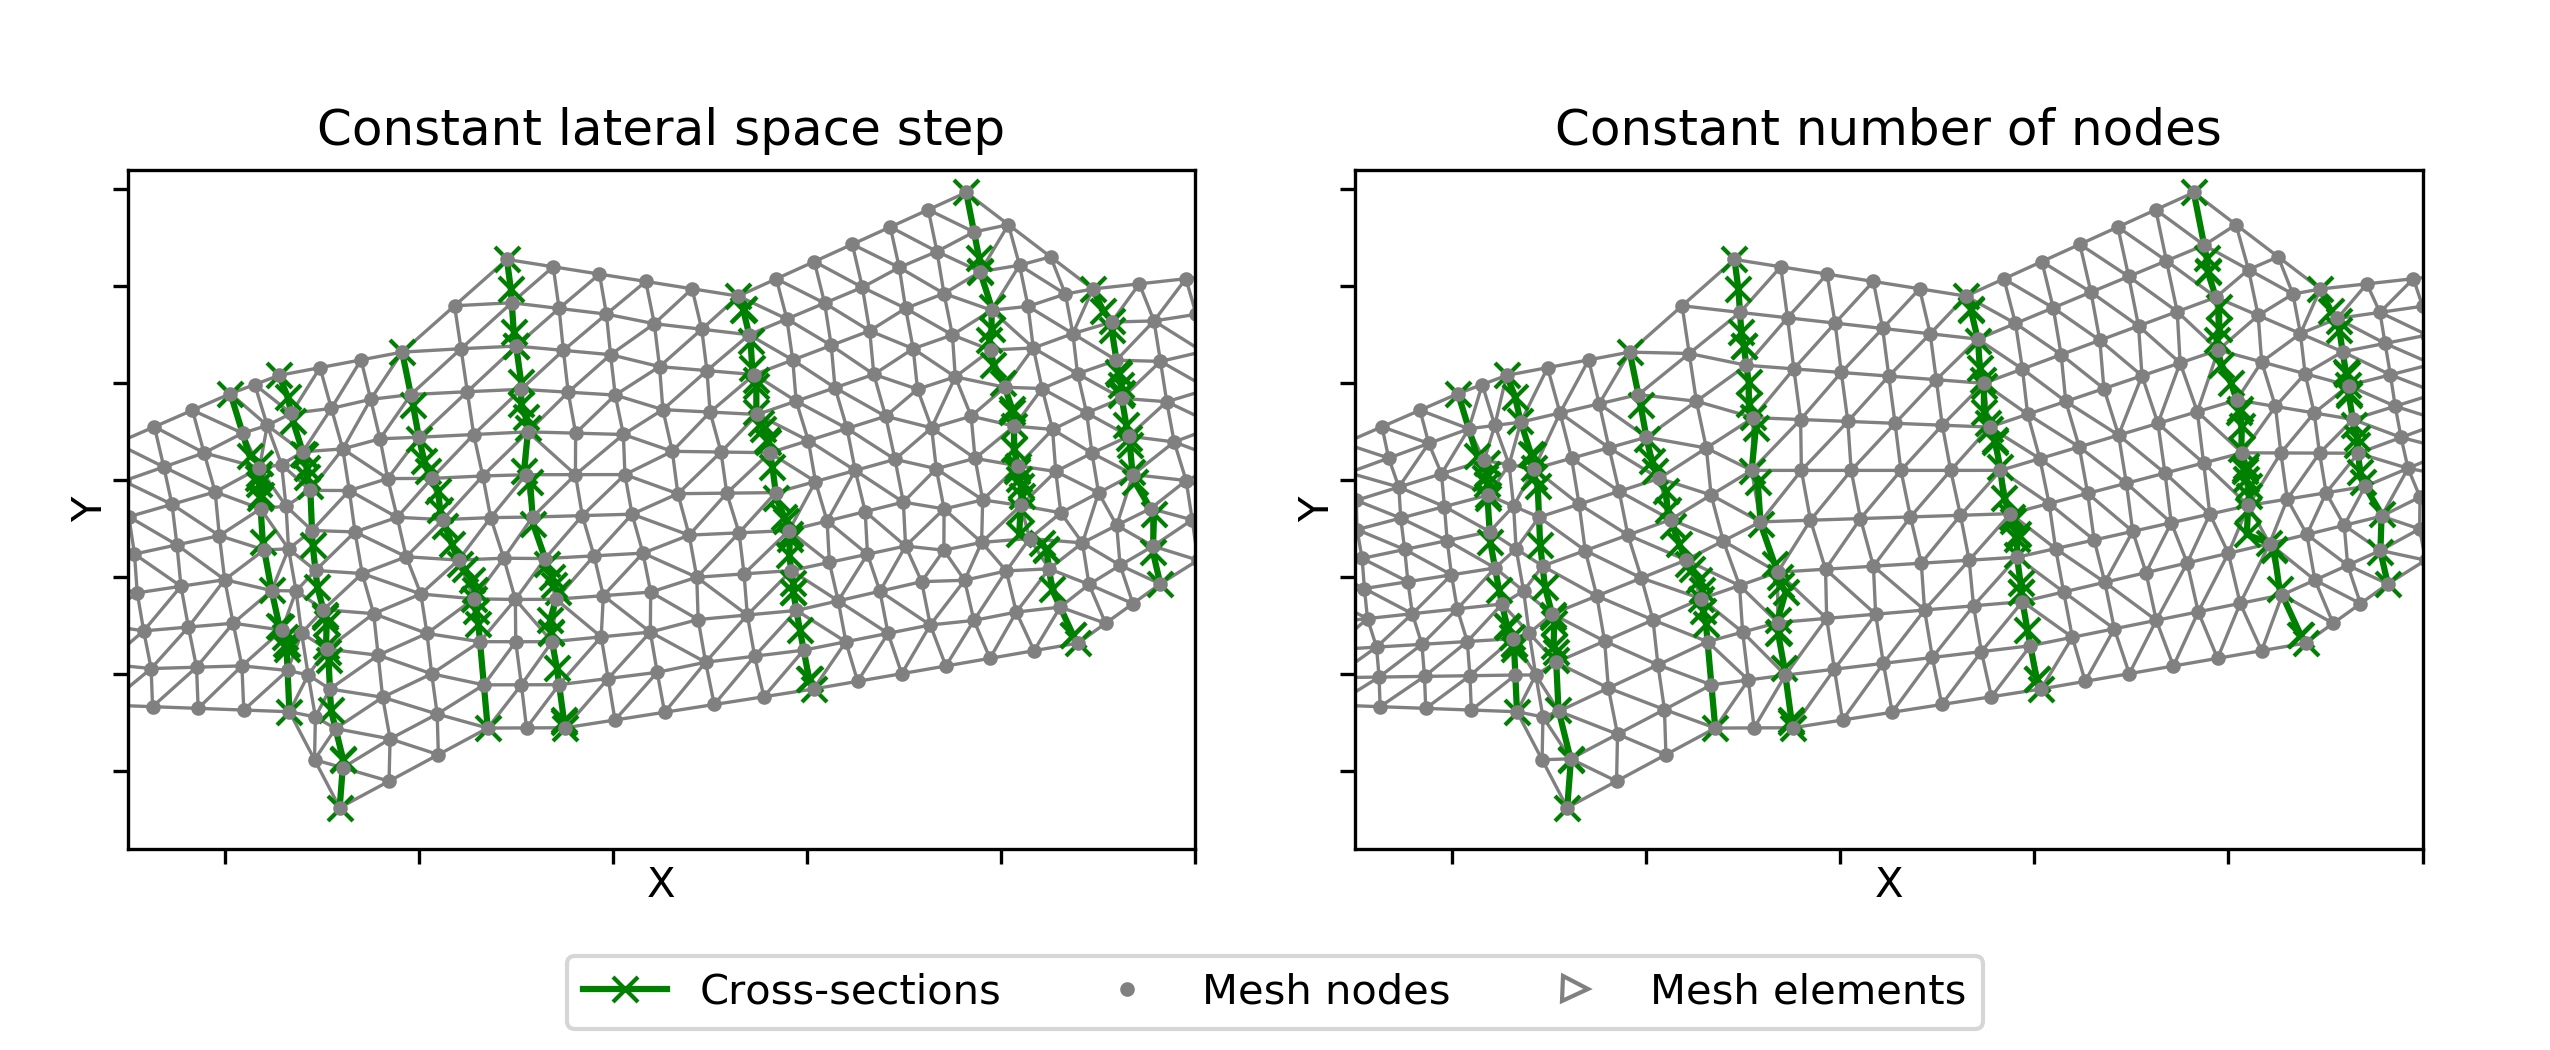
\includegraphics[width=12cm]{figures/plot_comp_lateral-discretization.png}}
\end{figure}

\end{frame}


\begin{frame}\frametitle{Feature 2: Constraint lines}

Guide the interpolation and follow topographic lines

\begin{figure}[H]
    \centerline{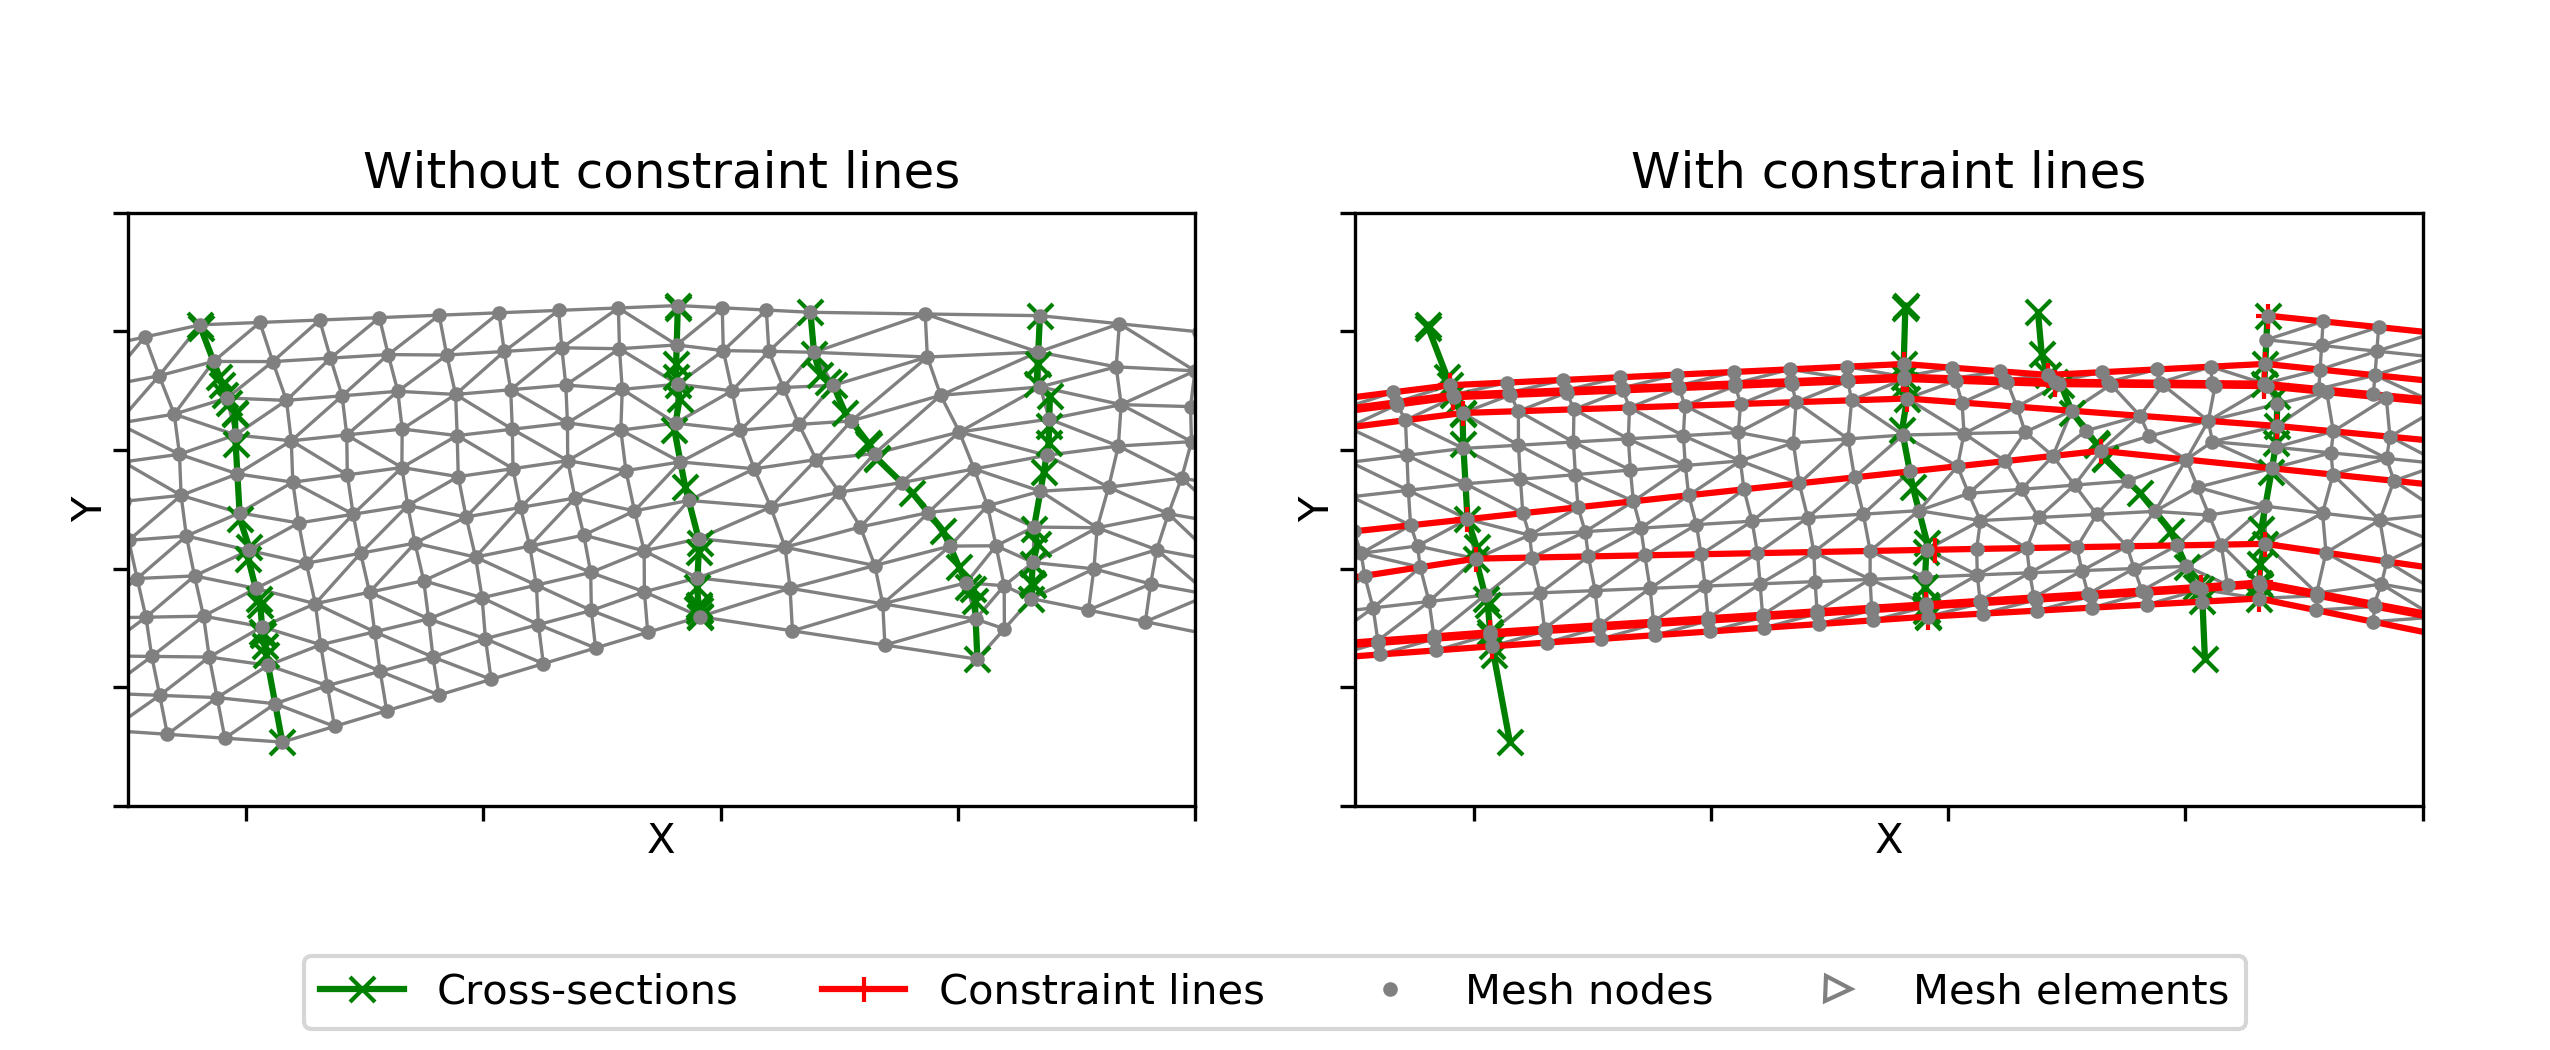
\includegraphics[width=12cm]{figures/plot_comp_constraint-lines.png}}
\end{figure}

\end{frame}


\begin{frame}\frametitle{Feature 3: XY coordinates interpolation of constraint lines}

\begin{figure}[H]
    \centerline{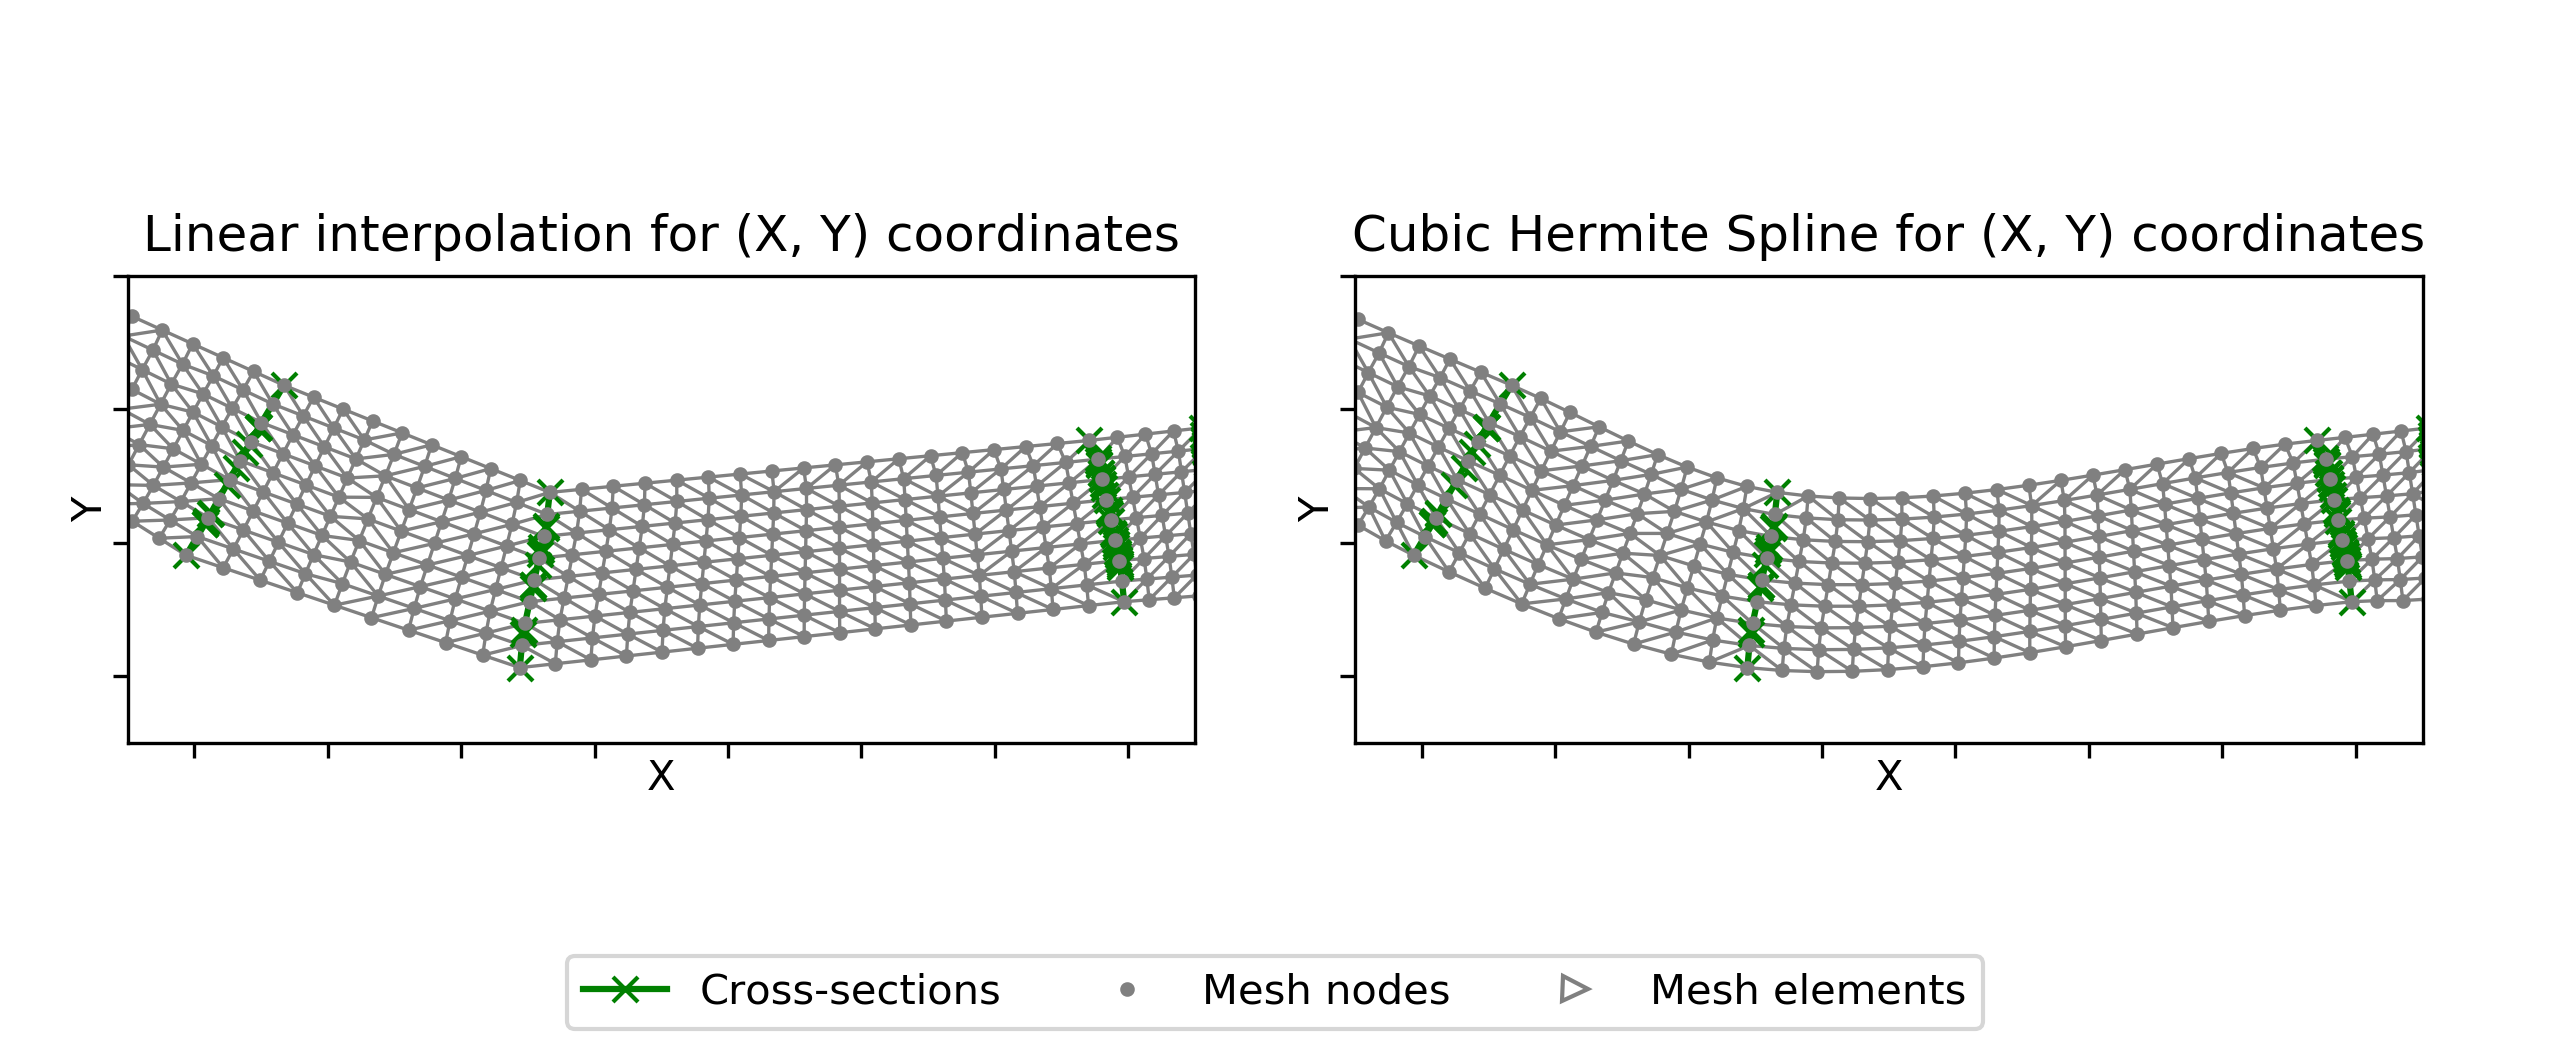
\includegraphics[width=12cm]{figures/plot_comp_xy-interp.png}}
\end{figure}

\end{frame}


\begin{frame}\frametitle{Feature 4: Flat projection of cross-section}

\begin{figure}[H]
    \centerline{    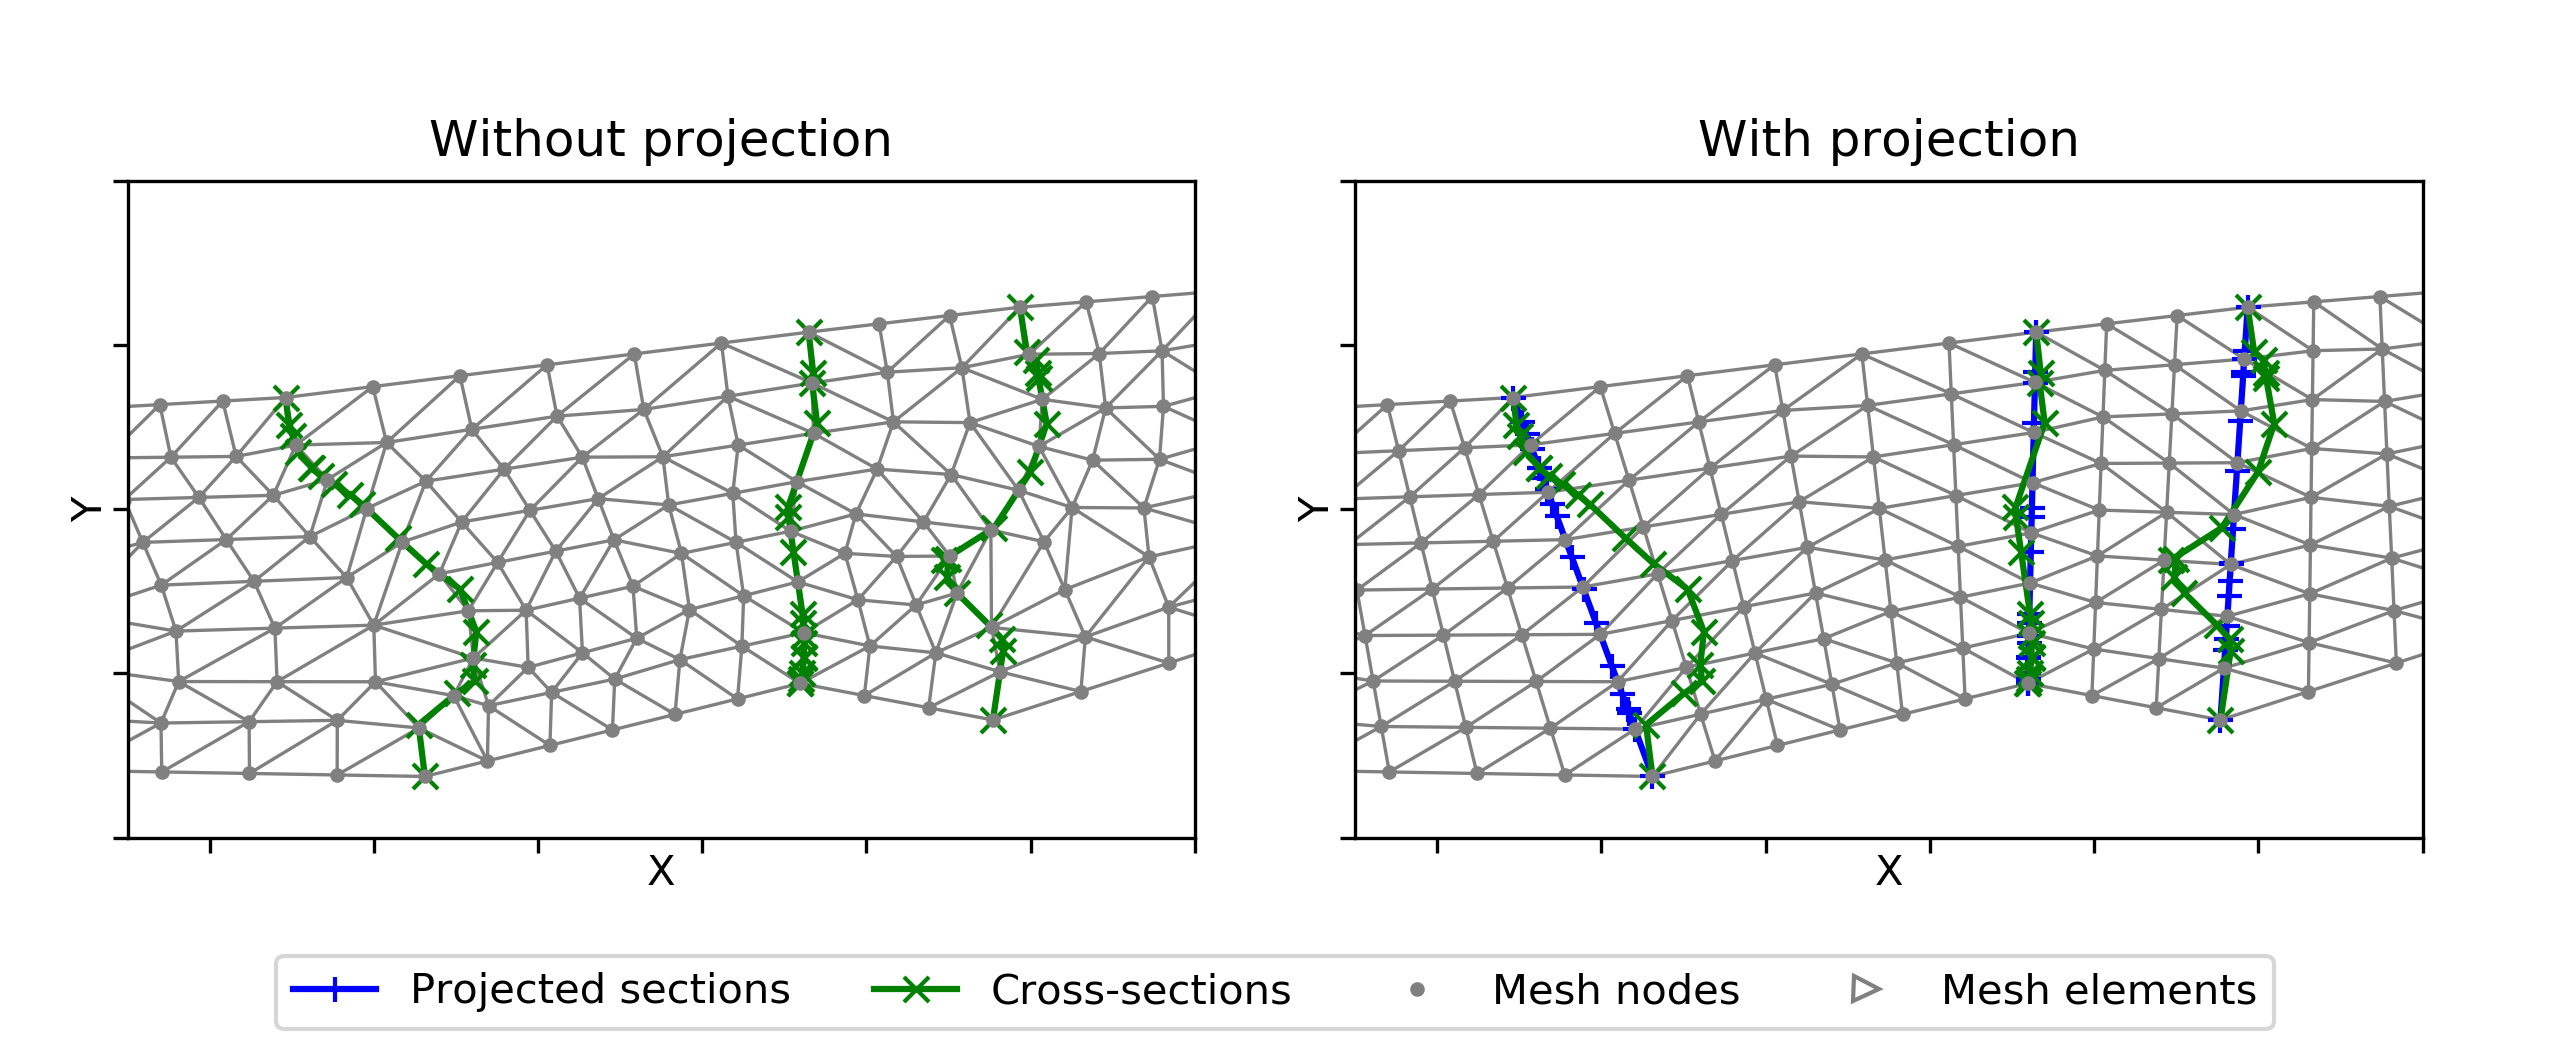
\includegraphics[width=12cm]{figures/plot_comp_project.png}}
\end{figure}

This option makes the elements mesh adjacent to the cross-sections more organized.

\end{frame}


%%%%%%%%%%%%%%%%%%%%%%%%%%%%%%%%%%%%%%%%%%%%%%%%%%%%%%%%%%%%%%%%%
\section{Interpolation}

\begin{frame}{Isotropic interpolation methods}

\vspace{-0.4cm}
\begin{figure}[H]
    \centering
        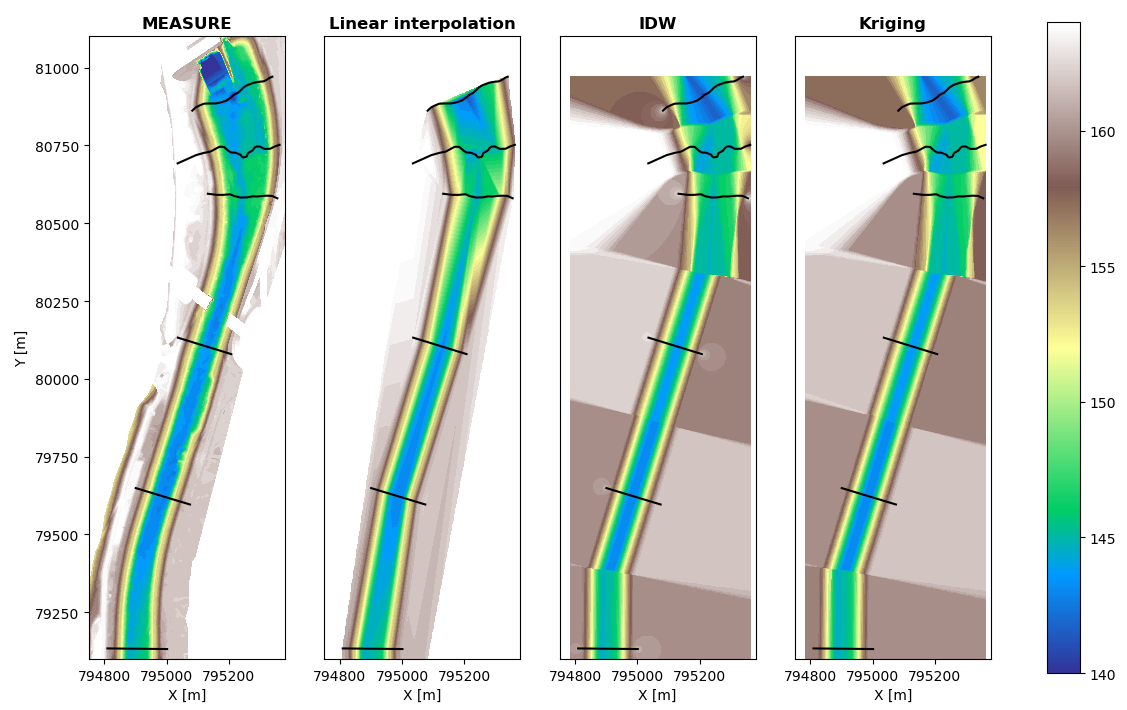
\includegraphics[width=0.8\textwidth]{figures/comp_isotropes.png}
        \caption{Bathymetry measured (left) compared to interpolated bathymetry from elevation along cross-sections (3 interpolation methods: Linear, IDW (Inverse distance weighting) and Kriging)}
\end{figure}

\end{frame}


\begin{frame}{Interpolation (of values at mesh nodes)}

  \begin{columns}[T,onlytextwidth]
    \column{0.52\textwidth}
\paragraphtitle{Consecutive 1D interpolators (lateral then longitudinal)}
Lateral interpolation methods:
\begin{itemize}
    \item \textbf{Linear}
    \item Akima spline
    \item Cubic spline
    \item PCHIP
\end{itemize}

Longitudinal interpolation method: \textbf{Linear}

\paragraphtitle{Global 2D interpolators}
\begin{itemize}
    \item Bilinear
    \item Bicubic
\end{itemize}

    \column{0.45\textwidth}
\begin{figure}[H]
    \centering
        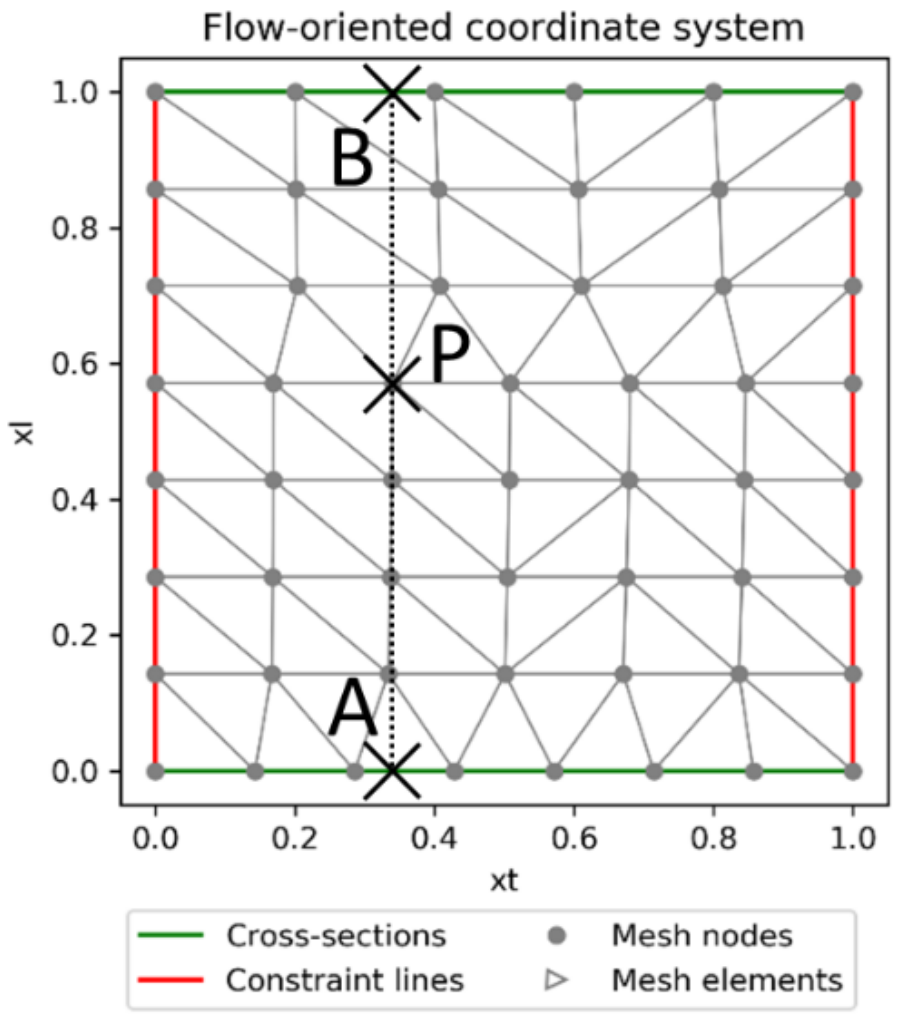
\includegraphics[height=5cm]{figures/plot_mesh_principle_6.png}
        \caption{Consecutive 1D interpolations to have values at node P}
\end{figure}
  \end{columns}

\end{frame}


\begin{frame}\frametitle{Validation test cases}
  \vspace{-0.5cm}
  \begin{columns}[T,onlytextwidth]
    \column{0.45\textwidth}
    \begin{figure}[H]
            \centering
            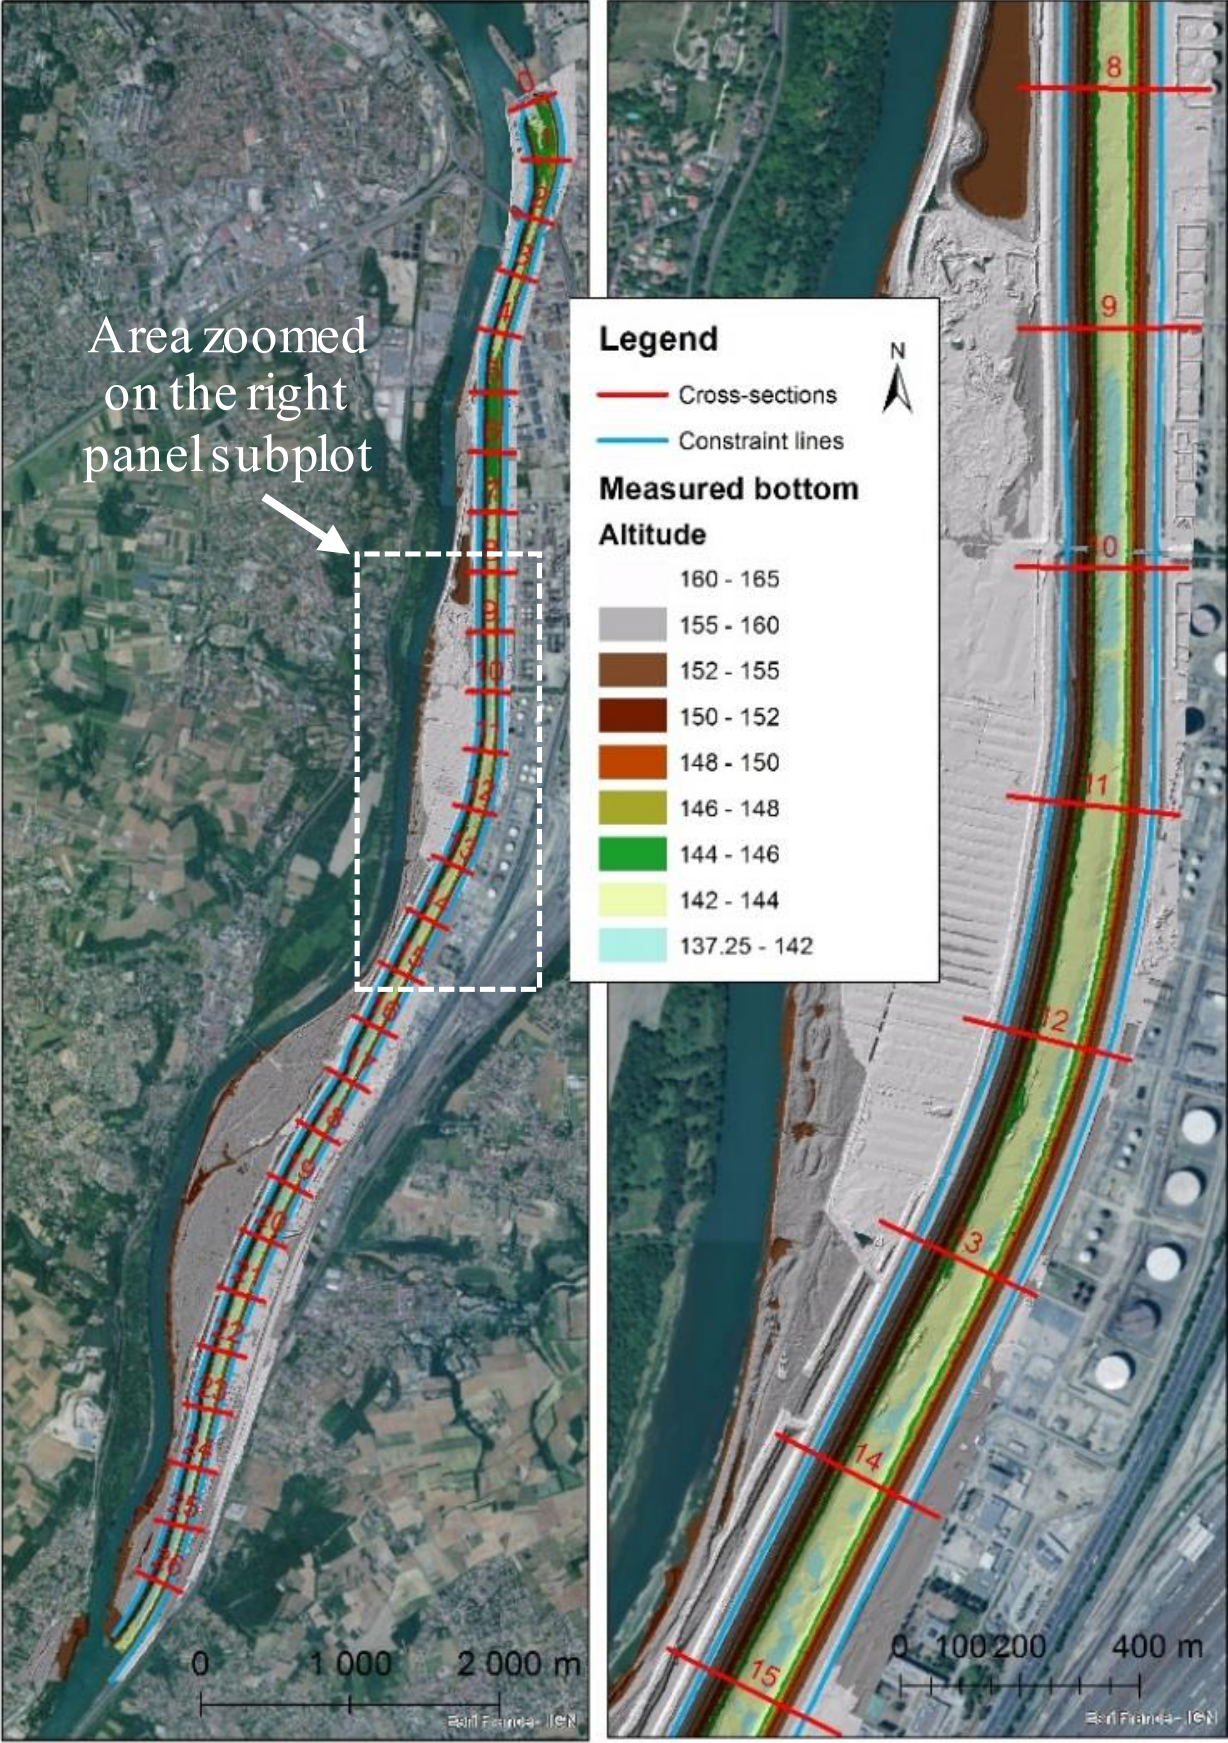
\includegraphics[height=6.4cm]{figures/map_VS.png}
        \caption{Study area: Vaugris (Rhône, France)}
    \end{figure}

    \column{0.45\textwidth}
    \begin{figure}[H]
            \centering
            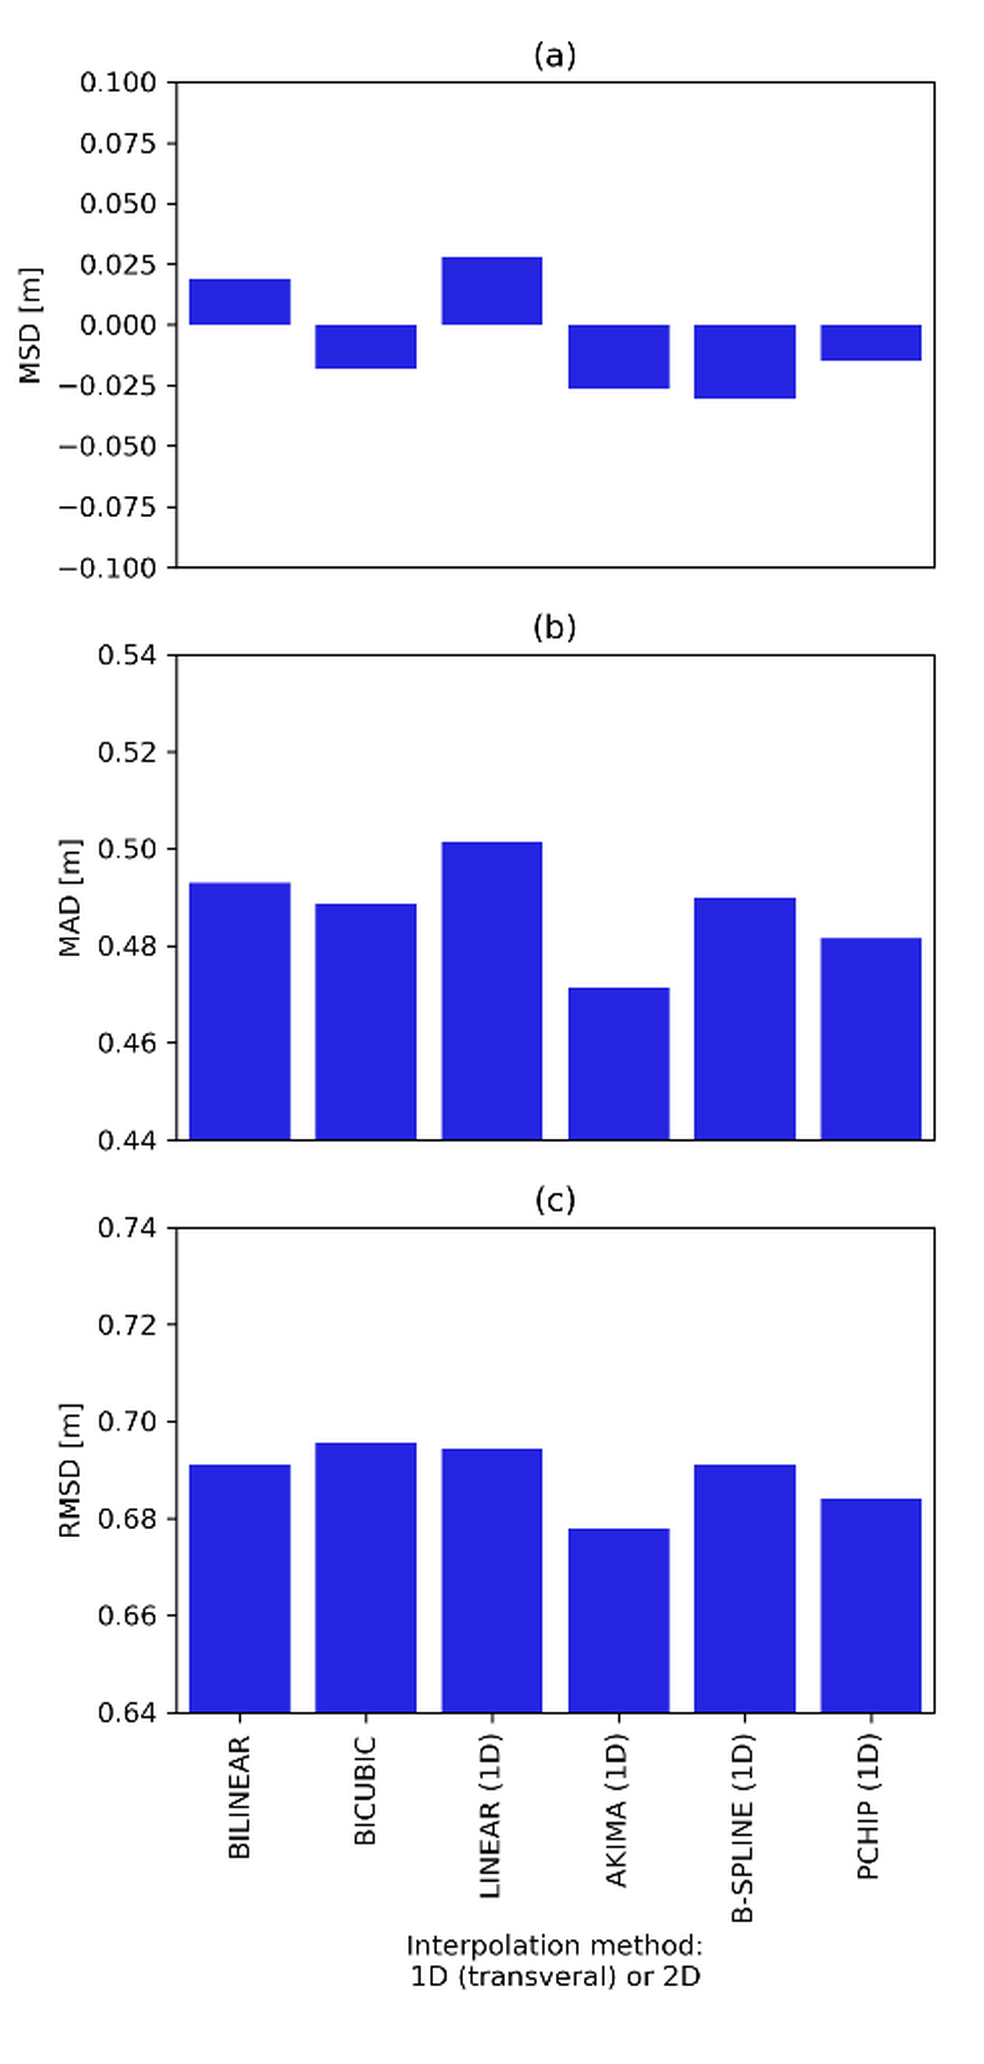
\includegraphics[height=6.4cm]{figures/criteria_VS.png}
        \caption{Criteria on difference in elevation (calculated - measured)}
    \end{figure}
  \end{columns}

\end{frame}


%%%%%%%%%%%%%%%%%%%%%%%%%%%%%%%%%%%%%%%%%%%%%%%%%%%%%%%%%%%%%%%%%
\section{Applications}

\begin{frame}{Channel mesher and intepolator}

\begin{figure}[H]
    \centering
    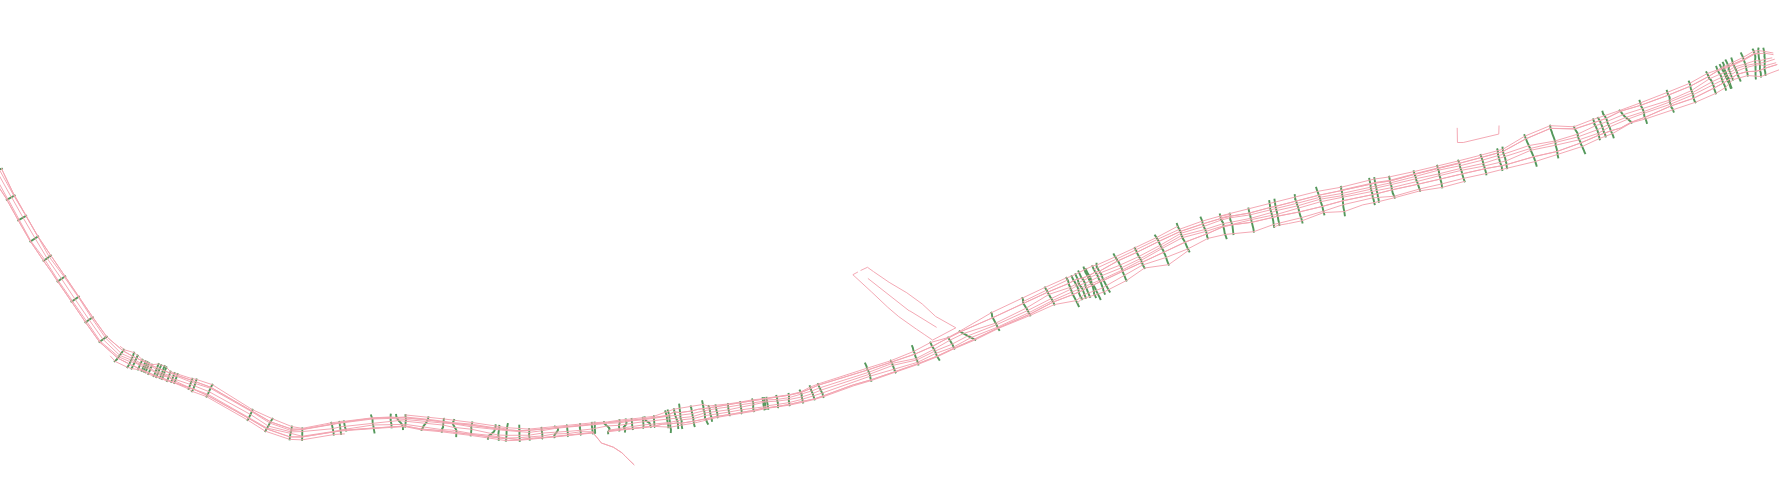
\includegraphics[width=\textwidth]{figures/leysse.png}
    \caption{Leysse river example}
\end{figure}

\end{frame}


\begin{frame}{Generate 2D surfaces from 1D model results}

\begin{itemize}
    \item Mesh over multiple branches
    \item Interpolation multiple frames and multiple variables:
        \begin{itemize}
            \item 1D variables: free surface elevation, Froude number...
            \item 2D variables: bottom elevation, friction coefficient, water depth, bed shear stress...
        \end{itemize}
\end{itemize}

  \begin{columns}[T,onlytextwidth]
    \column{0.3\textwidth}
    \begin{figure}[H]
            \centering
            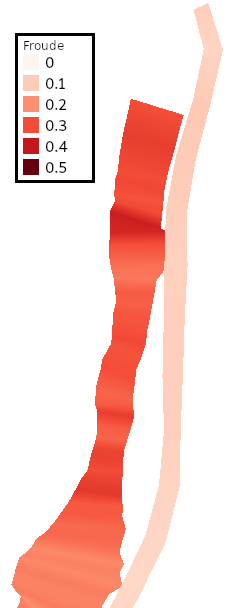
\includegraphics[height=4.1cm]{figures/mesh_crue10_run_froude.png}
        \caption{Froude Number (1D)}
    \end{figure}

    \column{0.65\textwidth}
    \begin{figure}[H]
            \centering
            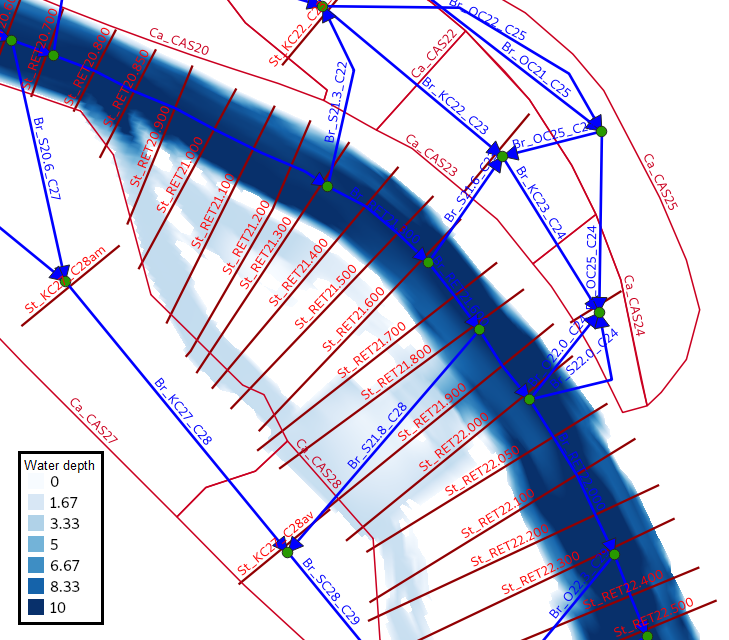
\includegraphics[height=4.1cm]{figures/mesh_crue10_run_hauteur_eau.png}
        \caption{Water depth (2D)}
    \end{figure}
  \end{columns}

\end{frame}


\section{Conclusion}

\begin{frame}{Conclusion and perspectives}

\begin{itemize}
    \item Open-source Python package
    \item Multiple aims
    \item Usefull for Mascaret-T2D coupling?
    \item Use in combinaison with BlueKenue or GMSH?
\end{itemize}

\end{frame}


{
  \setbeamertemplate{background}{}
  \setbeamertemplate{headline}{}
  \setbeamertemplate{footline}{}
  \setbeamercolor{background canvas}{bg=jauneCNR}
  \begin{frame}[c,noframenumbering]{}
    \begin{center}
          {\Large
        Thank you for your attention !

        \vspace{2cm}

        Any questions?
        }
    \end{center}
  \end{frame}
}


\lastframe


\appendix
%FIXME: Appendix frames numbering restarts from 1 (but progress bar remains full)

{
  \setbeamertemplate{background}{}
  \setbeamertemplate{headline}{}
  \setbeamertemplate{footline}{}
  \begin{frame}[c,noframenumbering]{\LARGE Appendix}
    % contenu vide
  \end{frame}
}


\begin{frame}

\begin{figure}[H]
    \centering
        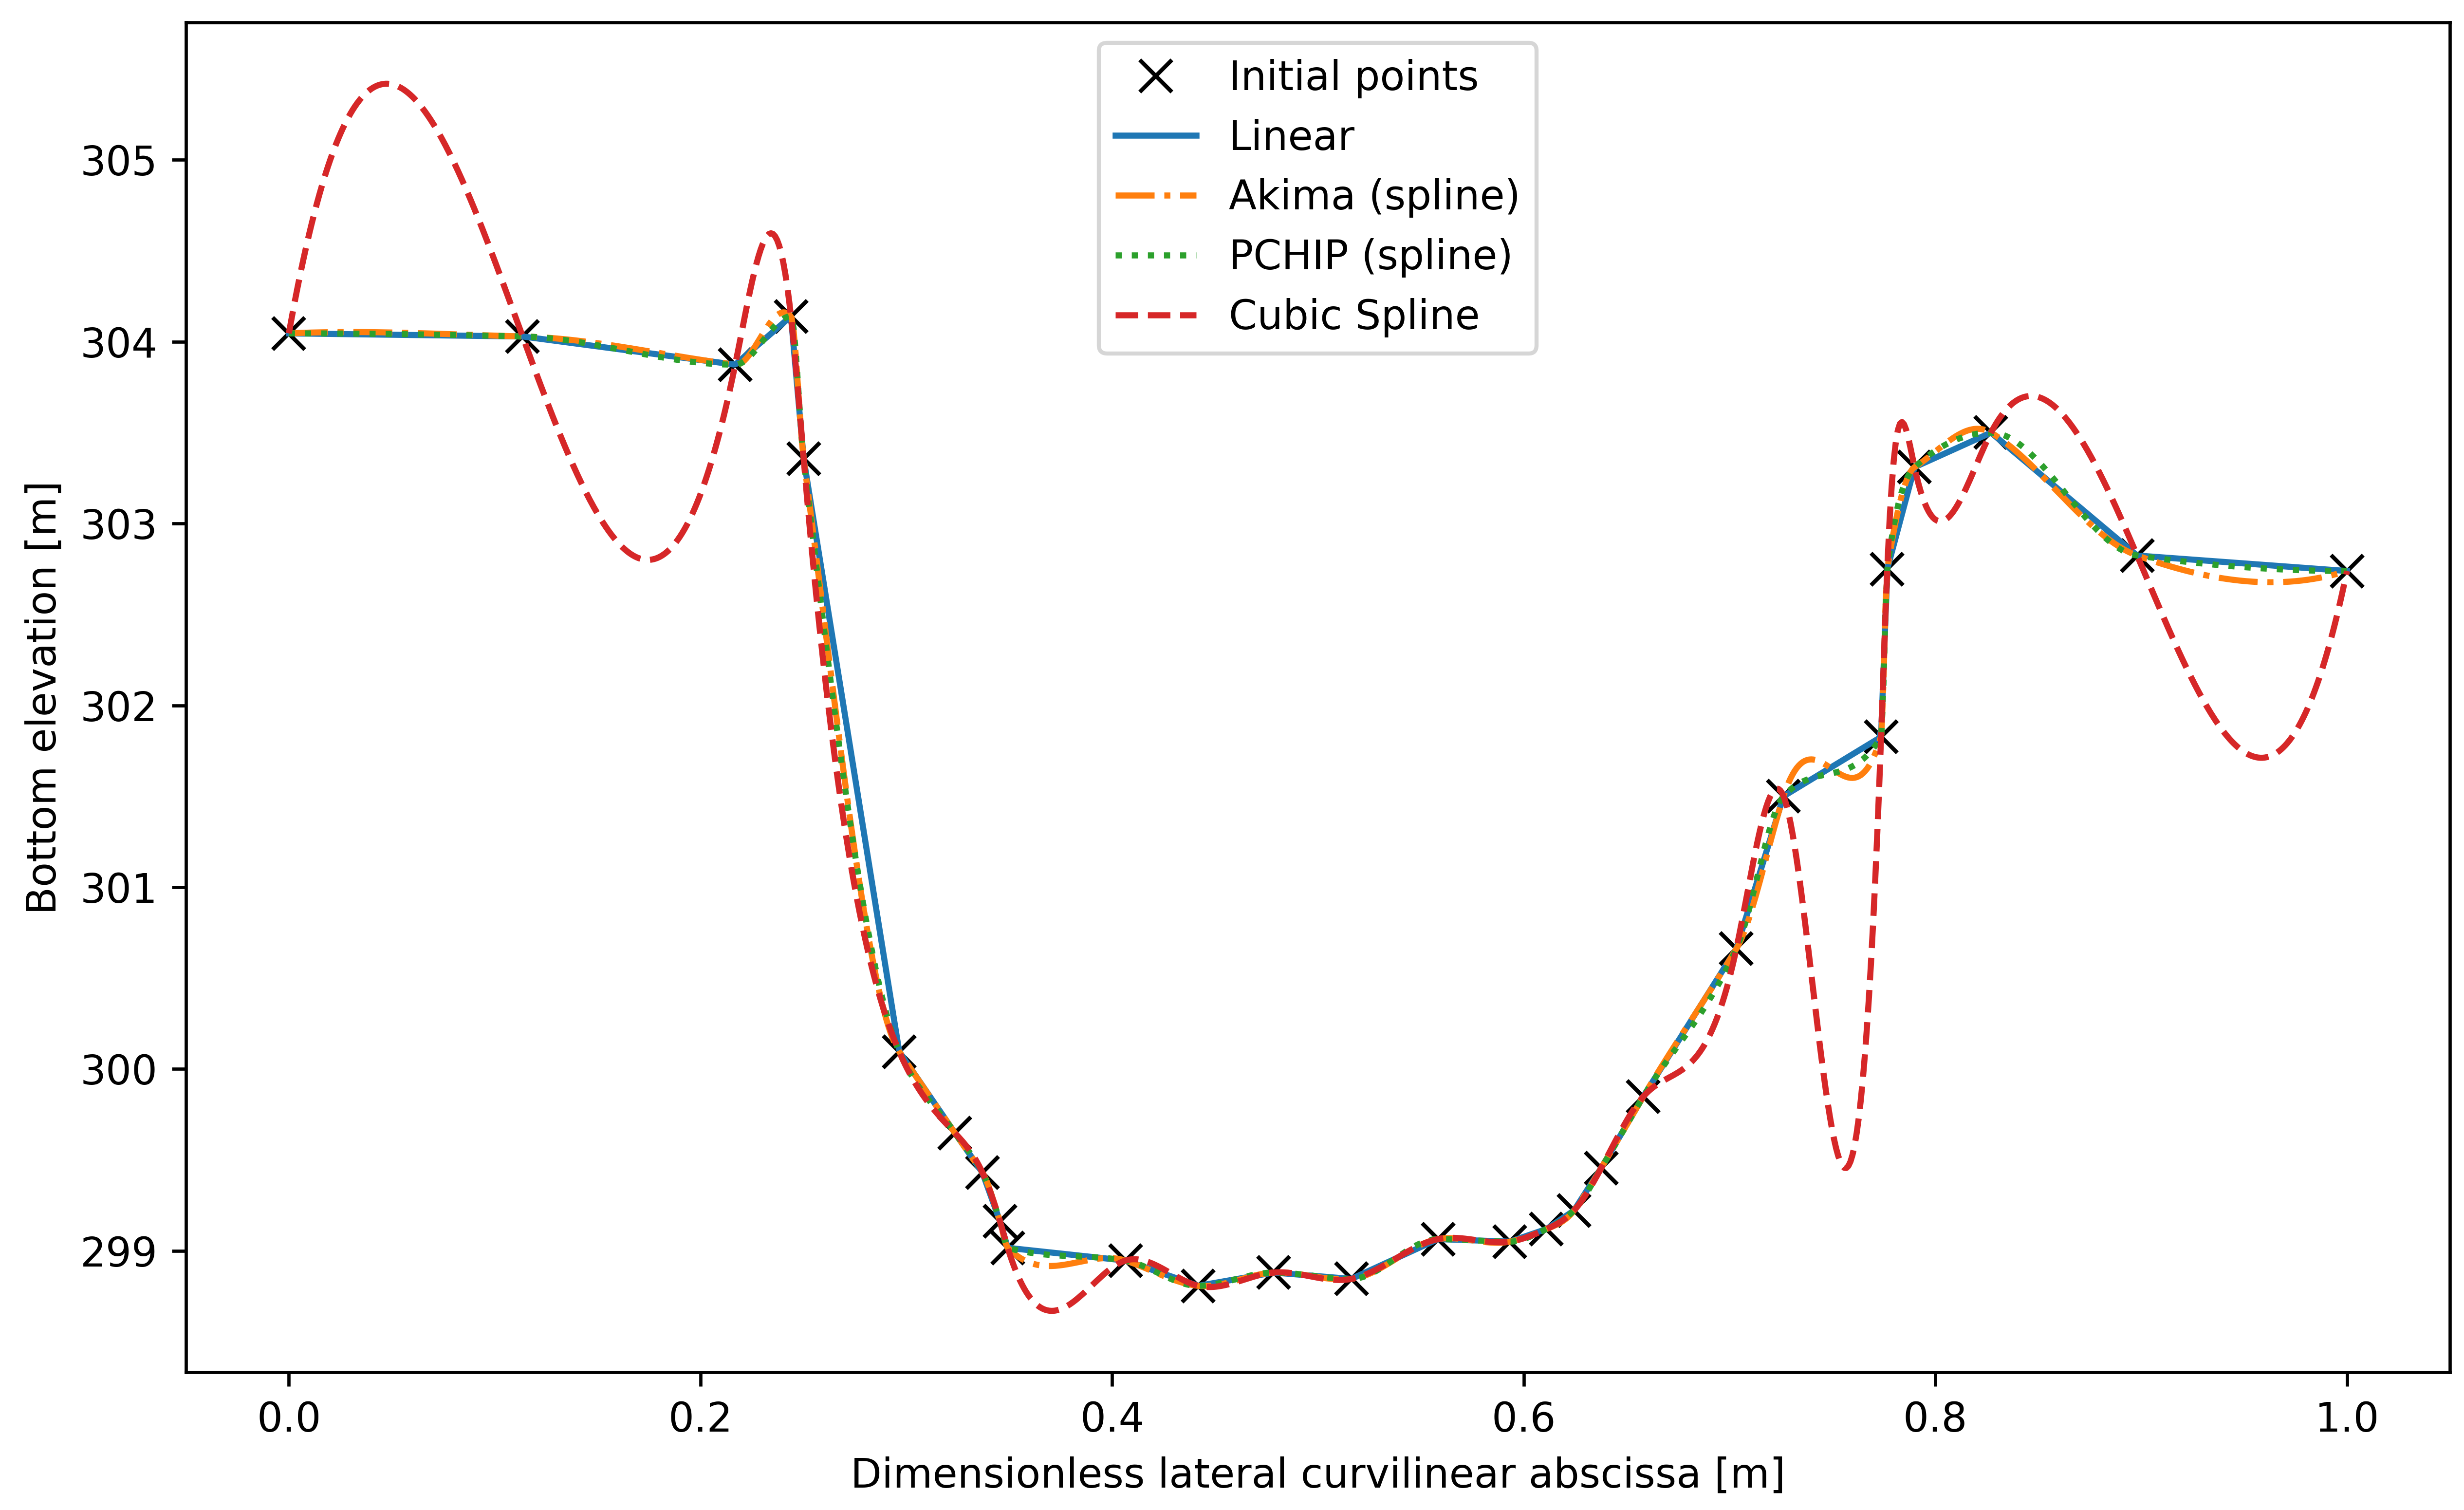
\includegraphics[width=0.7\textwidth]{figures/comp_lateral_interpolation.png}
        \caption{Comparison of linear, cubic spline, Akima and PCHIP interpolation at single cross section}
\end{figure}

Cubic spline is not robust. In the case of upsampling or non-equally spaced data, it creates over shooting at locations of abrupt changes in the slope.

\end{frame}


\begin{frame}{Mesh generation on L'Étournel site (1/2)}

A limited domain on the Upper Rhône River (upstream Génissiat dam) called L’Étournel is chosen to compare meshes generated with TatooineMesher with different space discretization options. This simple data set, presented in Figure below, includes 25 cross-sections intersected by at most 5 constraint lines.

\begin{figure}[H]
    \centering
    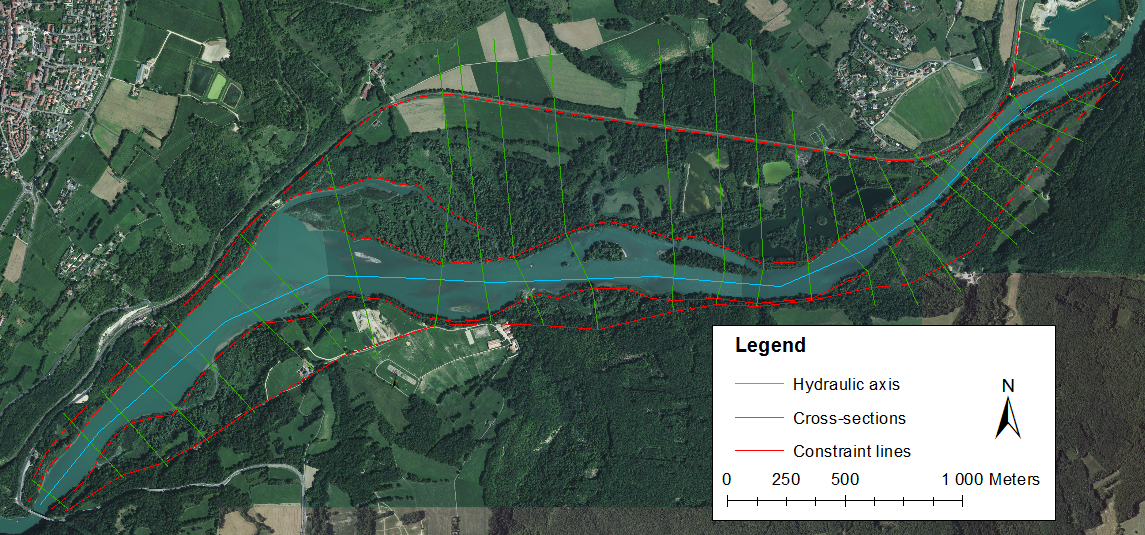
\includegraphics[width=8.5cm]{figures/map_Etournel.png}
    \caption{Geometrical data used to mesh “L’Étournel” site }
\end{figure}

\end{frame}


\begin{frame}\frametitle{Mesh generation on L'\'Etournel site (2/2)}

\begin{figure}[H]
    \centering
    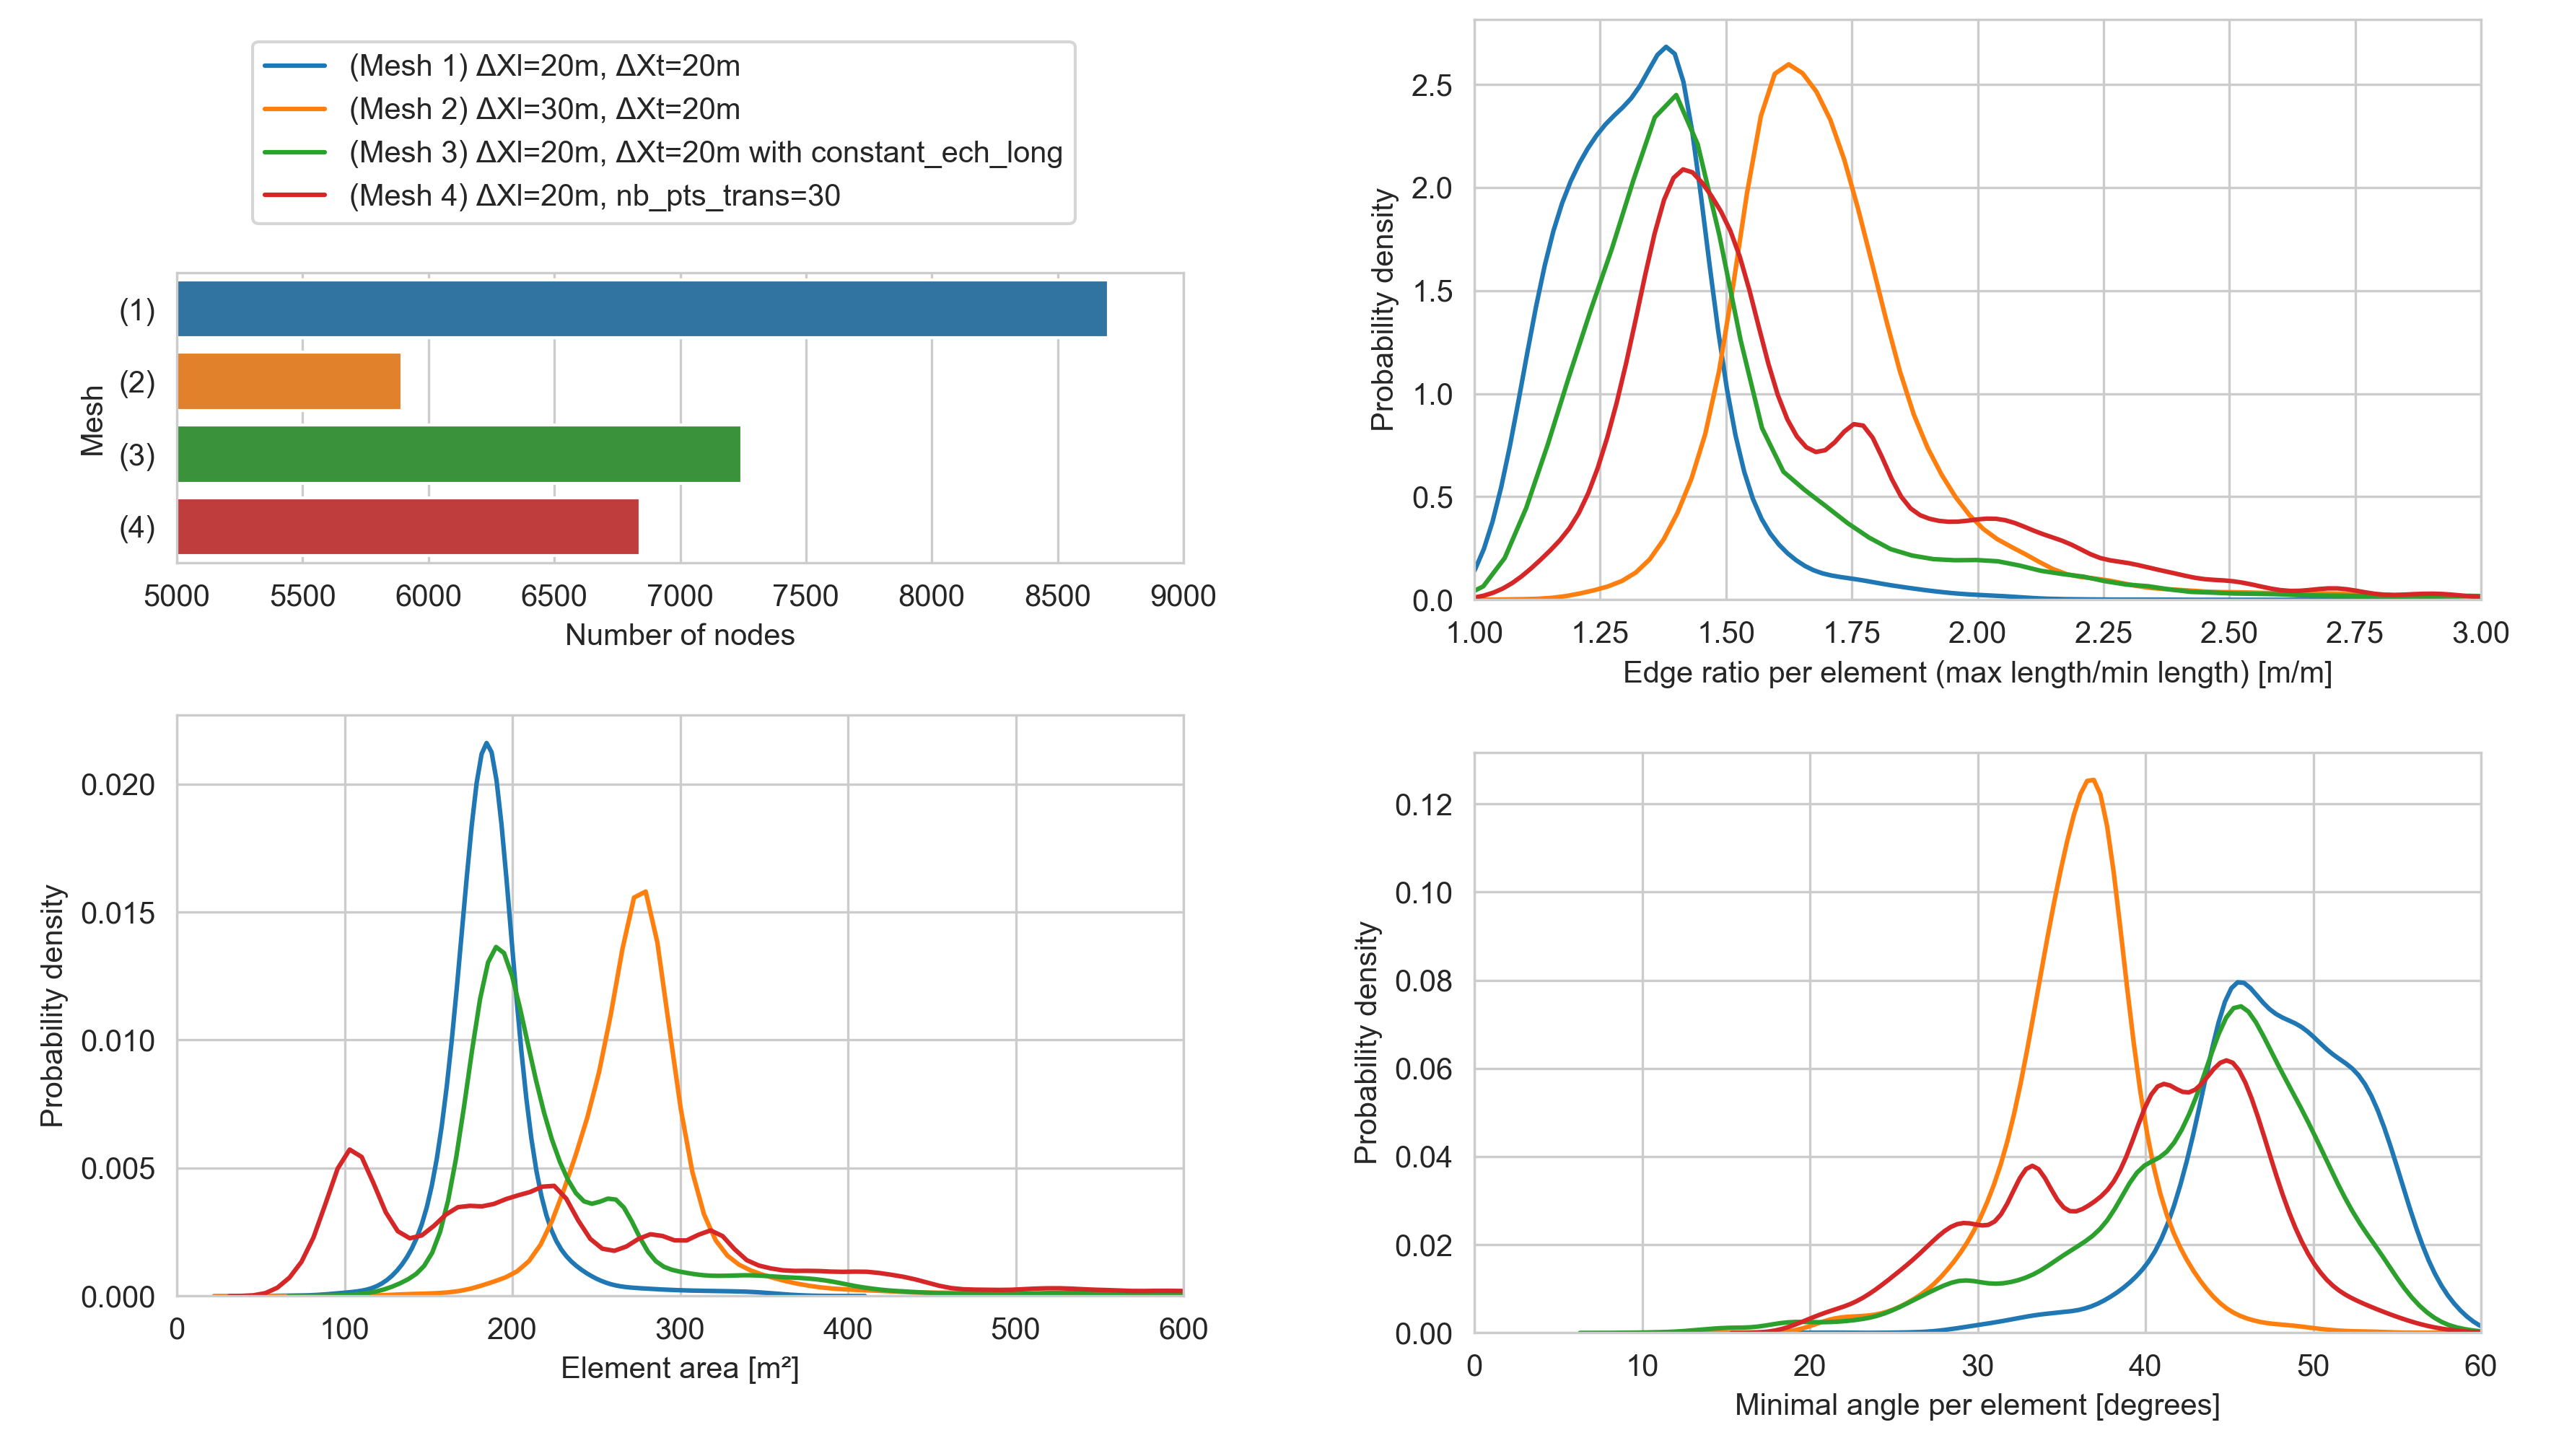
\includegraphics[width=10cm]{figures/etournel_result.png}
    \caption{Statistics on generated meshes}
\end{figure}

\end{frame}


%% \begin{frame}[allowframebreaks]{References}

%%   \bibliography{references}
%%   \bibliographystyle{abbrv}

%% \end{frame}


\sectionframe{The End...}{1.0}


\end{document}
